\documentclass{article}
\usepackage{anyfontsize}
\usepackage[UTF8]{ctex} % 如果需要支持中文
\usepackage{fontspec} 
% \setCJKmainfont{SourceHanSansCN-Light}[
%     BoldFont=SourceHanSansCN-Medium
% ]

\usepackage[a4paper, left=0.1in, right=0.1in, top=0.05in, bottom=0.05in]{geometry} % 设置四边页边距为0.1英寸{geometry} % 设置页边距为0.5英寸
\usepackage{enumitem} % 用于自定义列表
\usepackage{amsmath}  % 数学公式支持
\usepackage{hyperref} %不需要目录盒子注释这
\setlength{\parindent}{0pt} % 不缩进
\usepackage{etoolbox} % 用于列表操作
%调整类代码
\usepackage{comment}
\usepackage{tocloft} % 用于定制目录样式
%\usepackage{hyperref} %不需要目录盒子注释这
\usepackage{ifthen}
\usepackage{tikz}
\usepackage{titletoc}
\usepackage{graphicx}
\usepackage{amssymb}  % 提供数学符号，包括\therefore
%目录设定
%快捷键 CMD + / 注释
%  \renewcommand{\cftdot}{} % 隐藏目录中的页码
%  \cftpagenumbersoff{section}
%  \cftpagenumbersoff{subsection}
%  \makeatletter
%  \renewcommand{\@pnumwidth}{0em}  % 设置页码宽度为0
%  \renewcommand{\@tocrmarg}{0em}   % 设置右边距为0
%  \makeatother
 


\usepackage{environ}

\newif\ifshowcontent  % 定义一个条件判断变量
\showcontenttrue    % 设置为 false，隐藏所有 question 环境的内容

\newcounter{question} % 题目计数器
\setcounter{question}{0}
\NewEnviron{question}{%
    \ifshowcontent
        \par\stepcounter{question}\textbf{\thequestion.} \BODY\par % 如果显示内容，则输出
    \fi
}

\NewEnviron{choices}{%
    \ifshowcontent
        \begin{enumerate}[label=\Alph*., leftmargin=*]
            \BODY
        \end{enumerate}\par
    \fi
}

\NewEnviron{correctanswer}{%
    \ifshowcontent
        \textbf{答案:}\BODY\par
    \fi
}



\newenvironment{explanation}
{\textbf{解析:}\par}
{\par}



% 新增考察方面命令
\newcommand{\checklist}[1]{
    \textbf{考察:} #1 \par % 在题目下方显示考察方面
    \addcontentsline{toc}{subsection}{题号\thequestion 考察: #1} % 将考察内容添加到目录
    \vspace{2em} % 添加1em的垂直空间
}

\graphicspath{{images/}} %统一


\begin{document}
 %\fontsize{23}{31}\selectfont
 \tableofcontents % 添加目录
\newpage
%\pagestyle{empty}




\iftrue
\section{考点1:Measures of Financial Rlisk}
\setcounter{question}{0}
\begin{question}
    A quantitative analyst at a cryptocurrency trading firm is developing a risk model for digital assets. During a team meeting, she needs to explain why traditional risk models based on normal distribution might not be suitable for crypto assets. Which of the following statements about the return distributions of cryptocurrency investments is most likely correct?
    \\一位加密货币交易公司的量化分析师正在开发加密资产的风险模型。在团队会议上，她需要解释为什么传统的基于正态分布的风险模型不适合加密资产。以下哪个陈述关于加密货币投资的收益分布是最可能正确的？
    \end{question}
    
    \begin{choices}
        \item Machine learning models can accurately capture cryptocurrency returns by focusing solely on the mean return, as other parameters are less significant in digital asset markets.\\
        机器学习模型可以通过仅关注均值回报来准确捕捉加密货币回报，因为在数字资产市场中其他参数的重要性较低。
        \item The return distributions of cryptocurrency investments typically show thinner tails than traditional assets, making extreme price movements less frequent than in conventional markets.\\
        加密货币投资的收益分布通常表现出比传统资产更薄的尾部，使得极端价格波动发生的频率低于传统市场。
        \item Cryptocurrency returns tend to exhibit more pronounced peaks and fatter tails than the normal distribution would suggest, particularly during periods of market stress.\\
        加密货币回报倾向于表现出比正态分布更显著的峰值和更厚的尾部，特别是在市场压力期间。
        \item When applying normal distribution models to estimate potential losses in cryptocurrency trading, the probability of extreme events is typically overestimated compared to actual market behavior.\\
        当应用正态分布模型估计加密货币交易中的潜在损失时，极端事件的概率通常被高估，与实际市场行为相比。
    \end{choices}
    
    \begin{correctanswer}
    C
    \end{correctanswer}
    
    \begin{explanation}
        \textbf{A选项错误。}
        \begin{itemize}
            \item 即使使用先进的机器学习模型，仅依靠均值也无法充分描述加密货币收益的分布特征。收益分布的完整描述需要多个参数，包括但不限于均值、标准差、偏度和峰度。
        \end{itemize}
    
        \textbf{B选项错误。}
        \begin{itemize}
            \item 加密货币市场实际上表现出比传统资产更为显著的肥尾特征，极端价格波动的频率远高于正态分布预期，这反映了数字资产市场的高波动性特征。
        \end{itemize}
    
        \textbf{C选项正确。}
        \begin{itemize}
            \item 加密货币收益分布通常表现出显著的高峰肥尾特征，这意味着小幅波动和极端事件的发生频率都高于正态分布预期。这种特征在市场压力期间尤为明显，反映了数字资产市场的独特风险特征。
        \end{itemize}
    
        \textbf{D选项错误。}
        \begin{itemize}
            \item 使用正态分布模型估计加密货币市场的极端损失时，实际上会低估而非高估极端事件的概率，这是由于实际市场中肥尾现象的存在。
        \end{itemize}
    \end{explanation}
    
    \checklist{对比不同金融资产的收益率分布。（高峰肥尾现象）}



    \begin{question}
        A financial analyst evaluates a trading portfolio and determines that the Value at Risk (VaR) at a 95\% confidence interval for a 1-day holding period is \$500,000. Which of the following statements is TRUE?
        \\一位金融分析师评估了一个交易组合，并确定在95\%的置信水平下，持有期为1天的价值风险（VaR）为500,000美元。以下哪个陈述是正确的？
        \end{question}
        
        \begin{choices}
            \item The probability of the daily loss on the portfolio exceeding \$500,000 is 5\%.\\
            投资组合每日损失超过500,000美元的概率是5\%。
            \item There is a 95\% confidence that the daily loss on the portfolio will not exceed \$500,000.\\
            有95\%的信心认为投资组合每日损失不会超过500,000美元。
            \item The maximum daily loss that the portfolio can incur is \$500,000.\\
            投资组合可能遭受的最大每日损失是500,000美元。
            \item 95\% of financial analysts agree that the maximum loss on the portfolio is \$500,000.\\
            95\%的金融分析师同意投资组合可能遭受的最大损失是500,000美元。
        \end{choices}
        
        \begin{correctanswer}
            B
        \end{correctanswer}
        
        \begin{explanation}
            \textbf{A选项错误。}
            \begin{itemize}
                \item VaR的定义是，在95\%的置信水平下，损失不会超过\$500,000。这意味着分析师有95\%的信心认为损失不会超过这个值，而不是说损失发生的概率就是5\%。
            \end{itemize}
            
            \textbf{B选项正确。}
            \begin{itemize}
                \item VaR表示在95\%的置信水平下，投资组合的每日损失不会超过\$500,000。这是VaR的核心定义，因此选项B是正确的。
            \end{itemize}
            
            \textbf{C选项错误。}
            \begin{itemize}
                \item VaR并不代表投资组合可能遭受的最大损失。它只是一个在特定置信水平下的估计，投资组合可能会遭受超过\$500,000的损失，但这种情况发生的概率较低。
            \end{itemize}
            
            \textbf{D选项错误。}
            \begin{itemize}
                \item VaR是基于统计计算的风险度量，与金融分析师的主观意见无关。95\%的金融分析师是否同意这一点并不影响VaR的定义。
            \end{itemize}
        \end{explanation}
        \checklist{VaR的定义（置信就是有信心认为）}
    


        \begin{question}
            A risk management team is discussing the implications of Value at Risk (VaR) for their investment strategies. Which of the following statements about VaR is NOT correct?
            \\一个风险管理团队正在讨论价值风险（VaR）对投资策略的影响。以下哪个陈述关于VaR是不正确的？
        \end{question}
        
        \begin{choices}
            \item VaR can account for the diversified holdings of a financial institution, reducing capital requirements.\\
            VaR可以考虑金融机构投资组合的多样化，从而减少资本要求。
            \item VaR(10\%) = \$0 indicates that a positive dollar return is likely to occur on 90 out of 100 days.\\
            VaR(10\%) = \$0表示在90\%的置信水平下，100天中有10天可能会出现损失超过0美元的情况。
            \item VaR(1\%) can be interpreted as the number of days in which the portfolio value will exceed a loss of 1\%.\\
            VaR(1\%)可以解释为投资组合价值超过1\%损失的天数。
            \item A major limitation of the VaR measure is the use of two arbitrary parameters: confidence level and holding period.\\
            VaR度量一个主要限制是使用两个任意参数：置信水平和持有期。
        \end{choices}
        
        \begin{correctanswer}
            C
        \end{correctanswer}
        
        \begin{explanation}
            \textbf{A选项正确。}
            \begin{itemize}
                \item VaR确实可以考虑金融机构投资组合的多样化，从而帮助确定在一定置信水平下，投资组合在特定时间内可能遭受的最大损失。这有助于金融机构更有效地分配资本，以覆盖潜在的风险。
            \end{itemize}
            
            \textbf{B选项正确。}
            \begin{itemize}
                \item VaR(10\%) = \$0表示在90\%的置信水平下，100天中有10天可能会出现损失超过0美元的情况。换句话说，有90\%的概率损失不会超过0美元，而不是说有90天会出现正的回报。但是题目说的是“indicates”，也有一种“可能”的意思，因此，选项B可以被视为正确。
            \end{itemize}
            
            \textbf{C选项错误。}
            \begin{itemize}
                \item VaR(1\%)表示在99\%的置信水平下，损失超过1\%的情况在100天中可能发生1天。它并不直接表示损失超过1\%的具体天数，而是表示在给定的置信水平下，损失超过1\%的最大可能天数。因此，选项C的描述是不准确的。
            \end{itemize}
            
            \textbf{D选项正确。}
            \begin{itemize}
                \item VaR的一个主要限制是它依赖于两个任意参数：置信水平和持有期。VaR的结果可能会因这些参数的选择而有所不同，限制了其在不同情境下的适用性和可靠性。
                \item 这些参数的选择会显著影响VaR的计算结果。例如，较高的置信水平（如99\%）会导致更高的VaR值，从而可能导致过度保守的资本要求；而较低的置信水平（如90\%）则可能低估潜在风险。
                \item 此外，持有期的选择也会影响VaR的结果。短期持有期可能无法充分反映长期投资的风险特征。
            \end{itemize}
        \end{explanation}
        \checklist{VaR的特点。（VaR的一个主要限制是它依赖于两个任意参数：置信水平和持有期）}
    




        \begin{question}
            When using the delta-normal method to calculate Value-at-Risk (VaR) for a linear portfolio, how would the presence of fat tails in the return distribution affect the estimated VaR?
            \\当使用delta-normal方法计算线性投资组合的价值风险（VaR）时，收益分布中存在肥尾现象会对估计的VaR产生什么影响？
        \end{question}
        
        \begin{choices}
            \item The estimated VaR would likely underestimate the actual VaR.\\
            估计的VaR可能会低估实际VaR。
            \item The estimated VaR would be equal to the actual VaR.\\
            估计的VaR等于实际VaR。
            \item The estimated VaR would likely overestimate the actual VaR.\\
            估计的VaR可能会高估实际VaR。
            \item  The estimated VaR cannot be accurately determined without additional information.\\
            估计的VaR无法准确确定，因为没有额外信息。
        \end{choices}
        
        \begin{correctanswer}
            A
        \end{correctanswer}
        
        \begin{explanation}
            \textbf{A选项正确。}
            \begin{itemize}
                \item 在存在肥尾现象的情况下，收益分布的尾部损失发生频率较高。使用delta-normal方法计算的VaR通常假设收益分布是正态的，这会导致对潜在极端损失的低估。因此，实际的VaR可能会高于估计的VaR，选项A的描述是正确的。
            \end{itemize}
        
            \textbf{B选项错误。}
            \begin{itemize}
                \item 由于肥尾现象的存在，估计的VaR不太可能与实际VaR相等，因此选项B是错误的。
            \end{itemize}
        
            \textbf{C选项错误。}
            \begin{itemize}
                \item 由于肥尾现象，估计的VaR通常会低于实际VaR，而不是高于，因此选项C是错误的。
            \end{itemize}
        
            \textbf{D选项错误。}
            \begin{itemize}
                \item 肥尾会导致对VaR的低估，因为它忽略了肥尾对VaR的既定影响。因此，这个选项是不正确的。
            \end{itemize}
        \end{explanation}
        \checklist{肥尾现象对VaR的影响。（肥尾会导致对VaR的低估）}
        


              \begin{question}
            A portfolio manager at a hedge fund is conducting a training session on risk measurement principles. While explaining the concept of consistent risk measures, she notices that some junior analysts have misconceptions about these measures. Which of the following statements represents a misconception about consistent risk measures?
            \\一位对冲基金的组合经理正在进行风险度量原则的培训。在解释一致风险度量的概念时，她注意到一些初级分析师对这些度量有误解。以下哪个陈述代表了对一致风险度量的误解？
        \end{question}
        
        \begin{choices}
            \item Monotonicity implies that if portfolio A consistently outperforms portfolio B, then \(\text{Risk}(A) < \text{Risk}(B)\).\\
            单调性意味着如果投资组合A持续优于投资组合B，则\(\text{Risk}(A) < \text{Risk}(B)\)。
            \item Subadditivity indicates that the risk of two combined portfolios will not exceed the sum of individual risks, i.e., \(\text{Risk}(A + B) \leq \text{Risk}(A) + \text{Risk}(B)\).\\
            次可加性意味着两个组合的风险之和不会超过各个组合风险的和，即\(\text{Risk}(A + B) \leq \text{Risk}(A) + \text{Risk}(B)\)。
            \item Homogeneity means that if the scale of portfolio A doubles, its risk measure should also double, i.e., \(\text{Risk}(2A) = 2\text{Risk}(A)\).\\
            齐次性意味着如果投资组合A的规模翻倍，其风险度量也应翻倍，即\(\text{Risk}(2A) = 2\text{Risk}(A)\)。
            \item Translation invariance implies that adding cash to a portfolio reduces its risk measure, but the reduction is not necessarily equal to the cash added.\\
            平移不变性意味着向投资组合中添加现金会减少其风险度量，但减少量不一定等于添加的现金。
        \end{choices}
        
        \begin{correctanswer}
            D
        \end{correctanswer}
        
        \begin{explanation}
            \textbf{A选项正确，不选。}
            \begin{itemize}
                \item 单调性确保风险度量与投资组合的表现一致，表现差的投资组合具有更高的风险度量。
            \end{itemize}
        
            \textbf{B选项正确，不选。}
            \begin{itemize}
                \item 次可加性确保组合的风险不会合理地增加。
            \end{itemize}
        
            \textbf{C选项正确，不选。}
            \begin{itemize}
                \item 齐次性确保风险度量与投资规模成比例，这符合风险度量的直观理解。
            \end{itemize}
        
            \textbf{D选项错误。}
            \begin{itemize}
                \item 根据平移不变性的定义，向投资组合中添加现金K应使风险度量精确减少K，而不是可能不相等。这是风险度量的一个关键性质，确保添加无风险资产会直接减少风险度量。
            \end{itemize}
        \end{explanation}
\checklist{风险度量的性质。（齐次性、次可加性、平移不变性）}
       


\begin{question}
    An investor has purchased a stock that is part of the S\&P 500 index. Considering the statistical characteristics of stock returns, which of the following traits is most likely to be exhibited by the returns of this stock compared to a normal distribution?
    \\一位投资者购买了S\&P 500指数的一部分股票。考虑到股票回报率的统计特征，以下哪个特征最有可能被该股票的回报率与正态分布相比？
\end{question}

\begin{choices}
    \item The return distribution has low kurtosis, indicating a shape that is flatter than a normal distribution.\\
    收益分布具有低峰度，表明其形状比正态分布更平坦。
    \item The return distribution is symmetric around zero, meaning the left and right sides of the distribution are balanced.\\
    收益分布关于零对称，意味着分布的左侧和右侧是平衡的。
    \item The return distribution lacks excess kurtosis, meaning the tails are similar to those of a normal distribution, with few extreme values.\\
    收益分布缺乏超额峰度，意味着尾部与正态分布相似，只有少数极端值。
    \item The return distribution is more extreme, with more extreme values likely to occur in both positive and negative directions.\\
    收益分布更极端，更极端值可能在正向和负向都可能发生。
\end{choices}

\begin{correctanswer}
    D
\end{correctanswer}

\begin{explanation}
    \textbf{A选项错误。}
    \begin{itemize}
        \item 实际上，股票回报率的分布往往比正态分布更尖峰（更高的峰度），意味着大多数回报率集中在均值附近，分布的形状比正态分布更为尖锐。
    \end{itemize}

    \textbf{B选项错误。}
    \begin{itemize}
        \item 股票回报率的分布通常表现出负偏度，即分布的左侧尾部更长，表明在不利市场条件下可能出现更大的损失。
    \end{itemize}

    \textbf{C选项错误。}
    \begin{itemize}
        \item 股票回报率的分布通常具有超额峰度，即分布的尾部比正态分布更厚，这意味着极端值（无论是正向还是负向的极端回报）出现的概率更高。
    \end{itemize}

    \textbf{D选项正确。}
    \begin{itemize}
        \item 股票回报率的分布倾向于具有更厚的尾部，这表明在正向和负向都有可能出现更多的极端值。这是由于金融市场的波动性和极端事件的潜在影响。
    \end{itemize}
\end{explanation}

\checklist{股票回报率的分布特征。（尖峰、负偏度、超额峰度）}



\begin{question}
    A risk manager at a global investment bank is evaluating different risk metrics for their trading portfolio. The team is debating whether to use Value at Risk (VaR) or Expected Shortfall (ES) as their primary risk measure for regulatory reporting and internal risk control.Which of the following statements about these two risk measures is correct?
    \\一位全球投资银行的风险经理正在评估不同的风险指标用于其交易组合。团队正在讨论是否使用价值风险（VaR）或预期短缺（ES）作为主要风险度量用于监管报告和内部风险控制。以下哪个陈述关于这两种风险度量是正确的？
    \end{question}
    
    \begin{choices}
    \item Expected Shortfall satisfies the portfolio diversification principle (sub-additivity), while VaR may show inconsistent results when aggregating portfolio risks.\\
    预期短缺满足投资组合多样化原则（次可加性），而VaR在汇总投资组合风险时可能显示不一致的结果。
    \item VaR and Expected Shortfall provide identical risk information since they both measure potential losses over a specified time horizon at a given confidence level.\\
    VaR和预期短缺提供相同的风险信息，因为它们都在指定时间范围内以给定置信水平衡量潜在损失。
    \item Both VaR and Expected Shortfall require the portfolio returns to follow a normal distribution to be valid risk measures.\\
    两种风险度量方法都要求投资组合收益服从正态分布才能有效。
    \item Expected Shortfall remains constant regardless of the confidence level chosen, while VaR varies with different confidence levels.
    \\预期短缺在选择置信水平时保持不变，而VaR随不同置信水平变化。
    \end{choices}
    
    \begin{correctanswer}
    A
    \end{correctanswer}
    
    \begin{explanation}
    \textbf{A选项正确。}
    \begin{itemize}
        \item Expected Shortfall满足风险度量的子可加性原则，这意味着分散化投资总能降低组合风险。而VaR可能出现两个子组合的风险之和小于组合总风险的异常情况，这违反了投资组合理论中分散化降低风险的基本原则。
    \end{itemize}
    
    \textbf{B选项错误。}
    \begin{itemize}
        \item 虽然两个指标都衡量潜在损失，但它们提供的信息不同。VaR只表示特定置信水平下的最大损失值，而Expected Shortfall则进一步告诉我们超过VaR时的平均损失大小，提供了更完整的尾部风险信息。
    \end{itemize}
    
    \textbf{C选项错误。}
    \begin{itemize}
        \item 这两种风险度量方法都不要求收益必须服从正态分布。它们可以应用于任何类型的收益分布，包括偏态分布和厚尾分布。正态分布假设只是为了简化计算过程。
    \end{itemize}
    
    \textbf{D选项错误。}
    \begin{itemize}
        \item Expected Shortfall和VaR都会随着置信水平的变化而变化。提高置信水平会导致VaR值增加，相应的Expected Shortfall也会随之改变，因为它是基于VaR以外损失的条件期望。
    \end{itemize}
    \end{explanation}
    
    \checklist{风险度量指标比较（重点是VaR和ES的特性差异）}


    \begin{question}
        A risk management team at a global investment firm is evaluating different risk measures to enhance their portfolio management strategies. During a meeting, the team discusses the advantages of expected shortfall (ES) over value at risk (VaR) in capturing tail risk. Which of the following is not a reason that expected shortfall (ES) is a more appropriate risk measure than value at risk (VaR)?
        \\一位全球投资公司的风险管理团队正在评估不同的风险指标以增强其投资组合管理策略。在会议上，团队讨论了预期短缺（ES）相对于价值风险（VaR）在捕捉尾部风险方面的优势。以下哪个不是预期短缺（ES）比价值风险（VaR）更合适的原因？
    \end{question}
    
    \begin{choices}
        \item For normal distributions, only ES satisfies all the properties of coherent risk measurements.\\
        对于正态分布，只有ES满足一致性风险度量的所有性质。
        \item For nonelliptical distributions, the portfolio risk surface formed by holding period and confidence level is more convex for ES.\\
        对于非椭圆分布，ES形成的投资组合风险曲面在持有期和置信水平上更凸。
        \item ES gives an estimate of the magnitude of a loss.\\
        ES提供了损失幅度的估计。
        \item ES has less restrictive assumptions regarding risk/return decision rules than VaR.\\
        ES对风险/收益决策规则的假设较少限制性，这使得它在不同市场条件下更具适用性。
    \end{choices}
    
    \begin{correctanswer}
        A
    \end{correctanswer}
    
    \begin{explanation}
        \textbf{A选项错误。}
        \begin{itemize}
            \item VaR和ES在正态分布下都满足一致性风险度量的所有性质。然而，当不满足正态性假设时，只有ES满足所有一致性风险度量的性质。因此，选项A的描述是不正确的。
        \end{itemize}
    
        \textbf{B选项正确。}
        \begin{itemize}
            \item 对于非椭圆分布，ES形成的投资组合风险曲面在持有期和置信水平上更凸。这意味着ES在处理复杂分布时提供了更好的风险评估。
        \end{itemize}
    
        \textbf{C选项正确。}
        \begin{itemize}
            \item ES提供了损失幅度的估计，而不仅仅是一个置信水平下的最大损失值。这使得ES在评估极端损失时更为有效。
        \end{itemize}
    
        \textbf{D选项正确。}
        \begin{itemize}
            \item ES在风险/收益决策规则方面的假设较少限制性，这使得它在不同市场条件下更具适用性。
        \end{itemize}
    \end{explanation}

\checklist{ES和VaR的特点。（ES在非正态分布中也满足一致性风险度量）}



\begin{question}
    A financial institution has determined that the Value-at-Risk (VaR) for a portfolio over a 1-day horizon is USD 200 million. Based on this information, which of the following statements is TRUE regarding the VaR over a 5-day horizon?
    \\一家金融机构确定了一个投资组合在1天持有期下的价值风险（VaR）为20000万美元。基于此信息，以下哪个陈述关于5天持有期下的VaR是正确的？
\end{question}

\begin{choices}
    \item The VaR over a 5-day horizon is USD 447 million if returns are independently and identically distributed.\\
    如果收益是独立同分布的，5天持有期下的VaR为44700万美元。
    \item The VaR over a 5-day horizon is USD 447 million if returns are not independently and identically distributed.\\
    如果收益不是独立同分布的，5天持有期下的VaR为44700万美元。
    \item The VaR over a 5-day horizon remains USD 200 million since VaR is independent of the time horizon.\\
    5天持有期下的VaR保持为20000万美元，因为VaR与时间范围无关。
    \item The VaR over a 5-day horizon is USD 40 million, regardless of the distribution of returns.\\
    5天持有期下的VaR为4000万美元，无论收益的分布如何。
\end{choices}

\begin{correctanswer}
    A
\end{correctanswer}

\begin{explanation}
    \textbf{A选项正确。}
    \begin{itemize}
        \item 根据时间平方根法则，假设收益是独立同分布的，5天的VaR可以通过1天的VaR乘以\(\sqrt{5}\)来计算。具体计算如下：
        \[
        \text{VaR}_{5\text{ days}} = \text{VaR}_{1\text{ day}} \times \sqrt{5} = 200 \text{ million} \times \sqrt{5} \approx 200 \text{ million} \times 2.236 = 447.21 \text{ million}
        \]
    \end{itemize}

    \textbf{B选项错误。}
    \begin{itemize}
        \item 虽然计算结果为447百万美元，但如果收益不是独立同分布的，使用时间平方根法则不再适用。这意味着在这种情况下，VaR的计算可能会低估或高估实际风险，因此选项B不正确。
    \end{itemize}
    
    \textbf{C选项错误。}
    \begin{itemize}
        \item VaR确实依赖于时间范围。1天的VaR不能简单地认为在5天内保持不变，因为风险会随着时间的延长而增加。
    \end{itemize}
    
    \textbf{D选项错误。}
    \begin{itemize}
        \item USD 40 million的计算没有依据，且未能反映VaR的实际风险水平。此选项没有考虑到VaR的计算方法和时间平方根法则。
    \end{itemize}
\end{explanation}
\checklist{时间平方根法则。（平方根法则前提是独立同分布）}



\begin{question}
    A risk analyst at a commodity trading firm is evaluating an options portfolio that has a two-day Value-at-Risk (VaR) of \$3 million. The analyst needs to determine the appropriate translation of this VaR to a ten-day horizon under normal market conditions. What would be the estimated VaR for the ten-day horizon?
    \\一位商品交易公司的风险分析师正在评估一个期权组合，该组合在2天持有期下的价值风险（VaR）为300万美元。分析师需要确定在正常市场条件下，将此VaR转换为10天持有期下的适当值。10天持有期下的估计VaR是多少？
\end{question}

\begin{choices}
    \item \$4.743 million \\
    4743000美元
    \item \$5.678 million \\
    5678000美元
    \item \$6.708 million \\
    6708000美元
    \item \$7.890 million \\
    7890000美元
\end{choices}

\begin{correctanswer}
    C
\end{correctanswer}

\begin{explanation}

    \textbf{步骤1：确定2天的VaR。}
    \begin{itemize}
        \item 根据题目，已知2天的VaR为：
        \[
        \text{VaR(2 days)} = 3,000,000
        \]
    \end{itemize}

   
    \textbf{步骤2：推导1天的VaR。}
    \begin{itemize}
        \item 使用时间平方根法则，VaR与时间的平方根成正比。根据理论公式：
        \[
        \text{VaR(n days)} = \text{VaR(1 day)} \times \sqrt{n}
        \]
        \item 对于2天的VaR，可以表示为：
        \[
        \text{VaR(2 days)} = \text{VaR(1 day)} \times \sqrt{2}
        \]
        \item 由此可以推导出1天的VaR：
        \[
        \text{VaR(1 day)} = \frac{\text{VaR(2 days)}}{\sqrt{2}} = \frac{3,000,000}{\sqrt{2}} \approx 3,000,000 \times 0.707 \approx 2,121,320
        \]
    \end{itemize}

    \textbf{步骤3：计算10天的VaR。}
    \begin{itemize}
        \item 然后，计算从1天到10天的转换因子：
        \[
        \text{因子(1到10天)} = \sqrt{10} \approx 3.162
        \]
        
        \item 将1天的VaR与计算得到的因子相乘，得到10天的VaR：
        \[
        \text{VaR(10 days)} = \text{VaR(1 day)} \times \text{因子(1到10天)}
        \]
        \[
        \text{VaR(10 days)} = 2,121,320 \times 3.162 \approx 6,708,000
        \]
    \end{itemize}

\end{explanation}
\checklist{时间平方根法则。（需要知道转换因子的思维）} 





\begin{question}
    A risk analyst at a major investment bank is preparing a training session for new employees about Value at Risk (VaR). During the preparation, she reviews several statements about VaR's characteristics and interpretations. Which of the following statements about VaR is CORRECT?
    \\一位大型投资银行的风险分析师正在准备一份关于价值风险（VaR）的培训课程。在准备过程中，她审查了几种关于VaR特征和解释的陈述。以下哪个陈述关于VaR是正确的？
\end{question}

\begin{choices}
    \item VaR calculations primarily focus on individual asset risks, with portfolio diversification effects having minimal impact on capital requirements for financial institutions.\\
    VaR计算主要关注单个资产风险，投资组合多样化效应对金融机构资本要求的影响最小。
    
    \item When a portfolio's VaR(10\%) equals \$0, this indicates the portfolio will maintain positive returns for 90 consecutive trading days.\\
    当一个投资组合的VaR(10\%)等于0时，这意味着投资组合将在90个连续交易日内保持正收益。
    
    \item VaR was originally developed by commercial banks as a tool to better estimate their economic capital requirements while accounting for portfolio diversification effects.\\
    VaR最初由商业银行开发，作为一种工具，更好地估计其经济资本需求，同时考虑投资组合多样化效应。
    
    \item VaR measures provide precise predictions of future portfolio losses through advanced statistical modeling techniques.\\
    VaR度量提供通过高级统计建模技术对未来投资组合损失的精确预测。
\end{choices}

\begin{correctanswer}
    C
\end{correctanswer}

\begin{explanation}
    \textbf{A选项错误。}
    \begin{itemize}
        \item VaR计算实际上充分考虑了投资组合的多样化效应，这是其核心优势之一。通过计入资产间的相关性，VaR能够反映分散化带来的风险降低效果，从而可能降低金融机构的资本要求。
    \end{itemize}

    \textbf{B选项错误。}
    \begin{itemize}
        \item VaR(10\%) = \$0的含义是在任何给定日期有90\%的概率获得正收益，而不是连续90天保持正收益。这种解释混淆了概率特征和时间序列的概念。
    \end{itemize}

    \textbf{C选项正确。}
    \begin{itemize}
        \item VaR确实最初是由商业银行开发，目的是为了在考虑投资组合多样化效应的情况下，更准确地估计经济资本需求。这种方法帮助银行更好地理解和管理其风险敞口。
    \end{itemize}

    \textbf{D选项错误。}
    \begin{itemize}
        \item VaR是一个统计概率工具，提供的是在特定置信水平下的潜在损失估计，而不是精确的损失预测。它的结果受到多个因素的影响，包括模型假设、数据质量和市场条件等。
    \end{itemize}
\end{explanation}

\checklist{VaR的基本特性和解释（重点是VaR的概率解释和应用目的）}


\begin{question}
    A portfolio manager at a global investment bank is conducting a training session for junior risk analysts. During the session, she notices that some analysts have misconceptions about Value at Risk (VaR). Which of the following statements represents a common misconception about VaR?
    \\一位全球投资银行的投资组合经理正在对初级风险分析师进行培训。在培训过程中，她注意到一些分析师对价值风险（VaR）有误解。以下哪个陈述代表了对VaR的常见误解？
\end{question}

\begin{choices}
    \item A 95\% VaR of \$10 million means there is a 5\% chance that the portfolio losses will exceed \$10 million over the specified time horizon.\\
    95\%的VaR为1000万美元意味着在指定时间范围内，投资组合损失超过1000万美元的概率为5\%。
    
    \item VaR can be used to compare risk levels across different trading desks, as it provides a standardized risk measure in monetary terms.\\
    VaR可以用于比较不同交易部门的风险水平，因为它提供了标准化的风险度量，以货币单位表示。
    
    \item When calculating portfolio VaR, correlation effects between different assets are considered, which typically results in a portfolio VaR less than the sum of individual VaRs.\\
    当计算投资组合VaR时，考虑不同资产之间的相关性，通常会导致投资组合VaR小于单个VaR的总和。
    
    \item If a trading desk reports a daily 99\% VaR of \$1 million, it means the desk will lose exactly \$1 million on its worst trading days.\\
    如果一个交易部门报告每日99\%的VaR为100万美元，这意味着该部门在其最糟糕的交易日内将损失正好100万美元。
\end{choices}

\begin{correctanswer}
    D
\end{correctanswer}

\begin{explanation}
    \textbf{A选项正确。} 
    \begin{itemize}
        \item 这是VaR置信水平的准确统计解释。95\%的置信水平意味着在95\%的情况下损失不会超过VaR值，而5\%的显著性水平(\(\alpha\))表示超过VaR值的概率。需要注意的是，时间维度（如日VaR、周VaR）的明确指定很重要，因为风险暴露会随时间变化。
    \end{itemize}

    \textbf{B选项正确。} 
    \begin{itemize}
        \item VaR确实提供了一个标准化的风险度量，可以用货币单位表示不同交易部门的风险水平。这种统一的度量方式使得风险管理者能够比较不同资产类别（如股票与债券）的风险水平，便于设定风险限额和进行资本分配，同时也有助于高层管理者了解整体风险状况。
    \end{itemize}

    \textbf{C选项正确。} 
    \begin{itemize}
        \item 这反映了投资组合理论的核心原则。当资产间的相关系数小于1时，可以获得多样化收益。组合VaR的计算需要考虑完整的方差-协方差矩阵，因此通常小于单个资产VaR的简单加总。例如，两个负相关资产的组合可以显著降低整体VaR水平。
    \end{itemize}

    \textbf{D选项错误。} 
    \begin{itemize}
        \item 这个说法混淆了VaR的基本概念。VaR是统计意义上的最小损失值，而不是确切的损失预测。99\%的置信水平意味着在1\%的情况下会出现超过VaR的损失，而这些损失可能远超VaR值。这也是为什么在实践中需要补充使用压力测试等其他风险管理工具。
    \end{itemize}
\end{explanation}

\checklist{VaR的基本概念（重点是统计解释、实际应用及其局限性）}








\begin{question}
    A risk analyst at a fixed-income investment firm is currently evaluating the potential risks associated with a bond position of \$15 million. The analyst notes that the modified duration of the bond is 4.2 years, and the annualized yield volatility is 1.5\%. Using the duration method and assuming that the daily return on the bond position is independently identically normally distributed, the analyst needs to calculate the 10-day holding period VaR of the position with a 99\% confidence interval, assuming there are 252 business days in a year.
    \\一位固定收益投资公司的风险分析师正在评估与1500万美元债券头寸相关的潜在风险。分析师注意到债券的修正久期为4.2年，年化收益率波动率为1.5\%。使用久期方法，假设债券头寸的每日收益是独立同分布的正态分布，分析师需要计算持有期为10天的VaR，假设一年有252个交易日，置信区间为99\%。
\end{question}

\begin{choices}
    \item \$450,123 
    \item \$425,678 
    \item \$392,456 
    \item \$367,890 
\end{choices}

\begin{correctanswer}
    D
\end{correctanswer}

\begin{explanation}
    
    \textbf{步骤1：计算每日VaR。}
    \[
    \text{VaR(dy)} = Z \times \sigma = 2.33 \times \frac{0.015}{\sqrt{252}} \approx 0.0092
    \]
    其中，\(Z\)为99\%置信区间的Z值（约为2.33），\(\sigma\)为年化收益波动率。年化收益波动率的计算公式为：
    \[
    \sigma = \text{Annualized Volatility} = \frac{\text{Daily Volatility}}{\sqrt{T}}
    \]
    这里，T是每年的交易日数量。

    \textbf{步骤2：计算10天的VaR。}
    \[
    \text{VaR(10 days)} = \text{Modified Duration} \times \text{Bond Position} \times \text{VaR(dy)}
    \]
    \[
    \text{VaR(10 days)} = 4.2 \times 15,000,000 \times 0.0092 \approx 367,890
    \]

    因此，选项D的描述是正确的，10天的VaR为\$367,890。
\end{explanation}
\checklist{VaR的计算。（注意年化波动率计算）}





\begin{question}
    Mixed Fund has a portfolio worth USD 12,428,000 that consists of 42\% of fixed income 
    investments and 58\% of equity investments. The 95\% annual VaR for the entire portfolio 
    is USD 1,367,000 and the 95\% annual VaR for the equity portion of the portfolio is USD 
    1,153,000. Assume that there are 250 trading days in a year and that the correlation 
    between stocks and bonds is zero. What is the 95\% daily VaR for the fixed income portion 
    of the portfolio? 
    \\Mixed Fund投资组合价值为12428000美元，其中42\%为固定收益投资，58\%为股权投资。整个投资组合的95\%年VaR为1367000美元，股权部分的95\%年VaR为1153000美元。假设一年有250个交易日，股票和债券的相关系数为0。固定收益部分的95\%日VaR是多少？
\end{question}

\begin{choices}
    \item USD 21,263 
    \item USD 46,445 
    \item USD 55,171 
    \item USD 72,635
\end{choices}

\begin{correctanswer}1
    B
\end{correctanswer}


\begin{explanation}
    \textbf{步骤1：确定已知数据和假设，理解对应的公式。}
    \begin{itemize}
        \item 投资组合的方差：
        \[
        \text{Var(Portfolio)} = \text{Var}(A) + \text{Var}(B)
        \]
        如果资产A和资产B是独立的，则投资组合的方差可以表示为各个资产方差的和。
    
        \item VaR与方差之间的关系可以表示为：
        \[
        \text{VaR} = k \cdot \sqrt{\text{Var}}
        \]
        
        \item 组合VaR的推导：
        \begin{itemize}
            \item 将方差的表达式代入VaR的公式中：
            \[
            \text{VaR}_{\text{portfolio}} = k \cdot \sqrt{\text{Var}(A) + \text{Var}(B)}
            \]
            
            \item 由于 \(\text{Var}(A) = \left(\frac{\text{VaR}_A}{k}\right)^2\) 和 \(\text{Var}(B) = \left(\frac{\text{VaR}_B}{k}\right)^2\)，我们可以得到：
            \[
            \text{VaR}_{\text{portfolio}} = k \cdot \sqrt{\text{Var}(A) + \text{Var}(B)}
            \]
            代入方差的表达式：
            \[
            \text{VaR}_{\text{portfolio}} = k \cdot \sqrt{\left(\frac{\text{VaR}_A}{k}\right)^2 + \left(\frac{\text{VaR}_B}{k}\right)^2}
            \]
            简化后得到：
            \[
            \text{VaR}_{\text{portfolio}} = \sqrt{\text{VaR}^2_A + \text{VaR}^2_B}
            \]
        \end{itemize}
    \end{itemize}


    \textbf{步骤2：计算固定收益部分的VaR。}
    
    根据VaR的平方和公式：
    \[
    \text{VaR}^2_{\text{portfolio}} = \text{VaR}^2_{\text{equity}} + \text{VaR}^2_{\text{fixed income}}
    \]
    
    将已知值代入公式：
    \[
    1,367,000^2 = 1,153,000^2 + \text{VaR}^2_{\text{fixed income}}
    \]

    计算：
    \[
    1,367,000^2 = 1,868,689,000,000
    \]
    \[
    1,153,000^2 = 1,327,609,000,000
    \]
    
    代入计算：
    \[
    1,868,689,000,000 = 1,327,609,000,000 + \text{VaR}^2_{\text{fixed income}}
    \]
    
    解出固定收益部分的VaR平方：
    \[
    \text{VaR}^2_{\text{fixed income}} = 1,868,689,000,000 - 1,327,609,000,000 = 541,080,000,000
    \]

    取平方根得到固定收益部分的年VaR：
    \[
    \text{VaR}_{\text{fixed income}} = \sqrt{541,080,000,000} \approx 734,357
    \]

    \textbf{步骤3：将年VaR转换为日VaR。}
    
    使用时间平方根法则将年VaR转换为日VaR：
    \[
    \text{VaR}_{\text{daily}} = \frac{\text{VaR}_{\text{fixed income}}}{\sqrt{250}} = \frac{734,357}{\sqrt{250}} \approx 46,445
    \]

  

\end{explanation}

\checklist{VaR的计算。（计算组合VaR）} 




\begin{question}
    Greenfield Investments is estimating a daily VaR for its equity portfolio currently valued at USD 1.2 billion. Using returns for the last 500 days (ordered in decreasing order, from highest daily return to lowest daily return), the daily returns are the following: 2.10\%, 1.95\%, 1.85\%, 1.80\%, \ldots, -1.75\%, -1.90\%, -1.95\%, -2.05\%, -2.15\%. At the 99\% confidence level, what is your estimate of the daily VaR using the historical simulation method? 
    \\Greenfield Investments正在估算其股权投资组合的每日VaR，目前价值为12亿美元。使用过去500天的收益数据（按从最高日收益到最低日收益的顺序排列），每日收益如下：2.10\%，1.95\%，1.85\%，1.80\%，\ldots，-1.75\%，-1.90\%，-1.95\%，-2.05\%，-2.15\%。在99\%的置信水平下，使用历史模拟法估算的每日VaR是多少？
    \end{question}
    
    \begin{choices}
        \item USD 24.00 million 
        \item USD 22.50 million 
        \item USD 20.00 million 
        \item USD 25.50 million
    \end{choices}
    
    \begin{correctanswer}
        A 
    \end{correctanswer}
    
    \begin{explanation}
        要估算99\%置信水平下的每日VaR，我们需要确定对应于最差1\%收益的回报。
    
        \textbf{步骤1：确定观察数量。}
        \begin{itemize}
            \item 由于有500天的收益数据，最差1\%对应于最低的5个收益（因为 \(500 \times 0.01 = 5\)）。
        \end{itemize}
    
        \textbf{步骤2：识别第5个最低收益。}
        \begin{itemize}
            \item 从排序的收益中，第5个最低的收益为-2.05\%。
        \end{itemize}
    
        \textbf{步骤3：计算VaR。}
        \begin{itemize}
            \item VaR的计算公式为：
            \[
            \text{VaR} = \text{投资组合价值} \times \text{收益率}
            \]
            \item 代入数值：
           \[
           \text{VaR} = 1,200,000,000 \times (-2.05\%) = -24,600,000
           \]
           \item 由于VaR通常以正数表示，我们取其绝对值：
           \[
           \text{VaR} = 24.60 \text{ million}
           \]
        \end{itemize}
        
    
    因此，根据计算结果，最接近的选项是USD 24.00 million。在99\%的置信水平下，估算的每日VaR为USD 24.00 million。
    \end{explanation}
    
    \checklist{VaR的计算。（从一堆数里面找出VaR）} 




    \begin{question}
        A risk analyst uses historical data from 1,500 days of profit/loss information to calculate a daily VaR at the 95th percentile, which amounts to USD 5 million. Loss observations beyond the 95th percentile are then used to estimate the conditional VaR. If the losses beyond the VaR level, in millions, are USD 6, USD 7, USD 10, USD 13, USD 15, USD 18, USD 21, USD 25, and USD 35, what is the conditional VaR? 
        \\一位风险分析师使用1500天的利润/损失信息历史数据，计算每日VaR的95百分位数，金额为5000万美元。超过95百分位数的损失观测值用于估计条件VaR。如果超过VaR水平的损失金额（以百万美元为单位）为6, 7, 10, 13, 15, 18, 21, 25, 和 35，条件VaR是多少？
    \end{question}
    
    \begin{choices}
        \item USD 10 million 
        \item USD 20 million 
        \item USD 15 million 
        \item USD 17 million
    \end{choices}
    
    \begin{correctanswer}
       C
    \end{correctanswer}
    
    \begin{explanation}
    
        \textbf{步骤1：确定VaR水平。}
        \begin{itemize}
            \item 已知的VaR为USD 5 million，表示在95\%的置信水平下，损失不会超过这个值。
        \end{itemize}
        
        \textbf{步骤2：收集超出VaR的损失数据。}
        \begin{itemize}
            \item 超出VaR水平的损失数据为：USD 6, USD 7, USD 10, USD 13, USD 15, USD 18, USD 21, USD 25, 和 USD 35。
        \end{itemize}
        
        \textbf{步骤3：计算条件VaR。}
        \begin{itemize}
            \item 条件VaR是超出VaR水平的损失的平均值。我们需要计算这些损失的总和，然后除以损失的数量。
           
            - 计算步骤如下：
            \[
            \text{总损失} = 6 + 7 + 10 + 13 + 15 + 18 + 21 + 25 + 35 = 125
            \]
            - 计算损失的数量：
            \[
            \text{损失数量} = 9
            \]
            - 计算条件VaR：
            \[
            \text{条件VaR} = \frac{\text{总损失}}{\text{损失数量}} = \frac{125}{9} \approx 13.89 \text{ million}
            \]
        \end{itemize}
        
        \textbf{步骤4：选择最接近的选项。}
        \begin{itemize}
            \item 根据计算结果，条件VaR约为USD 13.89 million，最接近的选项是USD 15 million。
        \end{itemize}
        
        因此，条件VaR为USD 15 million。
    \end{explanation}
    
    \checklist{VaR的计算。（从一堆数里面找出VaR）} 



    \begin{question}
        A risk manager at an investment firm is analyzing the potential losses of a portfolio over different time horizons. The manager has asked a quantitative analyst to calculate the Value at Risk (VaR) for 5-, 10-, 15-, and 20-day periods, assuming that daily returns are independently and identically normally distributed. The manager notices an inconsistency in the analyst’s calculations. Which one of the following VaRs for this portfolio is inconsistent with the others?
        \\一位投资公司的风险经理正在分析投资组合在不同时间范围内的潜在损失。经理要求量化分析师计算5天、10天、15天和20天持有期下的价值风险（VaR），假设每日收益是独立同分布的正态分布。经理注意到分析师的计算存在不一致。以下哪个投资组合的VaR与其他不一致？
    \end{question}
    
    \begin{choices}
        \item VaR(5-day) = USD 200.00M  
        \item VaR(10-day) = USD 316.23M  
        \item VaR(15-day) = USD 387.30M  
        \item VaR(20-day) = USD 447.21M  
    \end{choices}
    
    \begin{correctanswer}
        A
    \end{correctanswer}
    
    \begin{explanation}
        
        \textbf{A选项正确。}
        \begin{itemize}
            \item VaR(5-day) = 200 \(\Rightarrow\) 
            \[
            \text{VaR}(1\text{-day}) = \frac{200}{\sqrt{5}} \approx 89.44
            \]
        \end{itemize}
        
        \textbf{B选项错误。}
        \begin{itemize}
            \item VaR(10-day) = 316.23 \(\Rightarrow\) 
            \[
            \text{VaR}(1\text{-day}) = \frac{316.23}{\sqrt{10}} \approx 100
            \]
        \end{itemize}
              
        \textbf{C选项错误。}
        \begin{itemize}
            \item VaR(15-day) = 387.30 \(\Rightarrow\) 
            \[
            \text{VaR}(1\text{-day}) = \frac{387.30}{\sqrt{15}} \approx 100
            \]
        \end{itemize}
              
        \textbf{D选项错误。}
        \begin{itemize}
            \item VaR(20-day) = 447.21 \(\Rightarrow\) 
            \[
            \text{VaR}(1\text{-day}) = \frac{447.21}{\sqrt{20}} \approx 100
            \]
        \end{itemize}
    
    \end{explanation}
    
    \checklist{VaR的计算。（需要转换到VaR(1-day)）} 
    
    


    \begin{question}
        A risk manager calculates that the VaR of a trading portfolio at 95\% confidence level is 12.8 million dollars. Assuming returns follow a one-tailed normal distribution, what would be the closest value of VaR if the confidence level is increased to 99\%?
        \\一位风险经理计算出交易组合在95\%置信水平下的VaR为1280万美元。假设收益服从单尾正态分布，如果置信水平提高到99\%，VaR的最近值是多少？
    \end{question}
    
    \begin{choices}
        \item 8.5 million dollars\\
        850万美元
        \item 14.2 million dollars \\
        1420万美元
        \item 18.1 million dollars \\
        1810万美元
        \item 18.9 million dollars
        \item 18.9 million dollars \\
        1890万美元
    \end{choices}
    
    \begin{correctanswer}
        C
    \end{correctanswer}
    
    \begin{explanation}
        \textbf{步骤1：理解正态分布的标准分位数。}
        \begin{itemize}
            \item 95\%置信水平对应的标准正态分位数 \(\alpha_{95\%} = 1.645\)
            \item 99\%置信水平对应的标准正态分位数 \(\alpha_{99\%} = 2.326\)
        \end{itemize}
    
        \textbf{步骤2：理解VaR的比例关系。}
        \begin{itemize}
            \item VaR与置信水平的标准正态分位数成正比
            \[
            \frac{VaR_{99\%}}{VaR_{95\%}} = \frac{\alpha_{99\%}}{\alpha_{95\%}}
            \]
        \end{itemize}
    
        \textbf{步骤3：计算99\%置信水平下的VaR。}
        \begin{itemize}
            \item 代入数值计算：
            \[
            VaR_{99\%} = VaR_{95\%} \times \frac{2.326}{1.645}
            \]
            \[
            VaR_{99\%} = 12.8 \times \frac{2.326}{1.645} = 18.1 \text{ million dollars}
            \]
        \end{itemize}
    
    \end{explanation}
    
    \checklist{VaR在不同置信水平下的转换计算（重点是正态分布分位数的应用）}
    



    \begin{question}
        Sarah, the risk analyst at Quantum Investment Fund, is comparing the risk profiles of two cryptocurrency investment strategies. She collected the following information about the loss distribution of these strategies. Which risk measure would be most appropriate to differentiate their risk severity?
        
        \begin{center}
        \begin{tabular}{|c|c|}
        \hline
        \multicolumn{2}{|c|}{Loss distribution for Strategy A} \\
        \hline
        Probability & Loss Amount \\
        \hline
        $98.5\%$ & $\$15,000$ \\
        $1.5\%$ & $\$45,000$ \\
        \hline
        \end{tabular}
        \end{center}
        
        \begin{center}
        \begin{tabular}{|c|c|}
        \hline
        \multicolumn{2}{|c|}{Loss distribution for Strategy B} \\
        \hline
        Probability & Loss Amount \\
        \hline
        $99\%$ & $\$15,000$ \\
        $0.5\%$ & $\$250,000$ \\
        $0.5\%$ & $\$350,000$ \\
        \hline
        \end{tabular}
        \end{center}
        Sarah,量子投资基金的风险分析师，正在比较两种加密货币投资策略的风险特征。她收集了关于这些策略损失分布的信息。哪种风险度量最合适来区分它们的风险严重程度？
        \begin{center}
            \begin{tabular}{|c|c|}
            \hline
            \multicolumn{2}{|c|}{策略A的损失分布} \\
            \hline
            概率 & 损失金额 \\
            \hline
            $98.5\%$ & $\$15,000$ \\
            $1.5\%$ & $\$45,000$ \\
            \hline
            \end{tabular}
            \end{center}
            
            \begin{center}
            \begin{tabular}{|c|c|}
            \hline
            \multicolumn{2}{|c|}{策略B的损失分布} \\
            \hline
            概率 & 损失金额 \\
            \hline
            $99\%$ & $\$15,000$ \\
            $0.5\%$ & $\$250,000$ \\
            $0.5\%$ & $\$350,000$ \\
            \hline
            \end{tabular}
            \end{center}
        \end{question}
        
        \begin{choices}
            \item 98\% VaR
            \item 99\% VaR
            \item 98\% ES
            \item 99\% ES
        \end{choices}
        
        \begin{correctanswer}
        A
        \end{correctanswer}
        
        \begin{explanation}
            
            \textbf{步骤1：首先计算Strategy A的风险指标。}
            \begin{itemize}
                \item $98\%$ VaR = $\$15,000$
                \item $99\%$ VaR = $\$45,000$
                \item $98\%$ ES = $\frac{98.5}{98} \times \$15,000 + \frac{1.5}{98} \times \$45,000 = \$15,459$
                \item $99\%$ ES = $\$45,000$
            \end{itemize}
            
            \textbf{步骤2：然后计算Strategy B的风险指标。}
            \begin{itemize}
                \item $98\%$ VaR = $\$15,000$
                \item $99\%$ VaR = $\$250,000$
                \item $98\%$ ES = $\frac{99}{98} \times \$15,000 + \frac{0.5}{98} \times \$250,000 + \frac{0.5}{98} \times \$350,000 = \$18,163$
                \item $99\%$ ES = $\frac{1}{2} \times \$250,000 + \frac{1}{2} \times \$350,000 = \$300,000$
            \end{itemize}
            
            \textbf{步骤3：汇总比较。}
            \begin{center}
            \begin{tabular}{|c|c|c|}
            \hline
            指标 & Strategy A & Strategy B \\
            \hline
            $98\%$ VaR & $\$15,000$ & $\$15,000$ \\
            $99\%$ VaR & $\$45,000$ & $\$250,000$ \\
            $98\%$ ES & $\$15,459$ & $\$18,163$ \\
            $99\%$ ES & $\$45,000$ & $\$300,000$ \\
            \hline
            \end{tabular}
            \end{center}
            
            \textbf{步骤4：结论分析。}
            \begin{itemize}
                \item $98\%$ VaR能够最好地区分两个策略的风险，因为它显示了两个策略在正常市场条件下的风险水平是相同的。
                \item 其他指标（$99\%$ VaR、$98\%$ ES、$99\%$ ES）都显示Strategy B的风险明显高于Strategy A，这可能导致过度保守的风险评估。
            \end{itemize}
            \end{explanation}
        
        \checklist{风险度量指标的选择与计算（VaR和ES的比较分析）}
    




        \begin{question}
            Sarah, a quantitative analyst at XYZ Asset Management, is analyzing a structured product with returns following a uniform distribution between -25\% and 40\%. To assess the risk profile, she needs to calculate both VaR and ES at the 95\% confidence level. What are the 95\% VaR and 95\% ES for this product?
            \\Sarah,XYZ资产管理公司的量化分析师，正在分析一个收益率在-25\%和40\%之间均匀分布的结构性产品。为了评估风险特征，她需要在95\%的置信水平下计算VaR和ES。这个产品的95\%VaR和95\%ES是多少？
            \end{question}
            
            \begin{choices}
                \item 20.5\% and 22.75\%
                \item 21.75\% and 23.25\%
                \item 22.75\% and 21.5\%
                \item 21.5\% and 22.75\%
            \end{choices}
            
            \begin{correctanswer}
            D
            \end{correctanswer}
            
            \begin{explanation}
            \textbf{步骤1：理解均匀分布的特征}
            \begin{itemize}
                \item 收益率范围：[-25\%, 40\%]
                \item 分布长度：65\% (从-25\%到40\%)
                \item 均匀分布意味着每个点的概率密度相等
            \end{itemize}
            
            \textbf{步骤2：计算95\% VaR}
            \begin{itemize}
                \item 使用均匀分布的分位数公式： $\frac{x-(-25\%)}{40\%-(-25\%)} = 1-95\% = 5\%$，得到$x = -21.75\%$
                \item 因此，95\% VaR = 21.5\%
            \end{itemize}
            
            \textbf{步骤3：计算95\% ES}
            \begin{itemize}
                \item ES是VaR以外区域的平均损失，在均匀分布中，这等于VaR点和最小值的平均值。
                \item 因此，$ES = \frac{-25\% + (-21.5\%)}{2} = -22.75\%$
            \end{itemize}
            
            \textbf{步骤4：图形说明}
            \begin{center}
                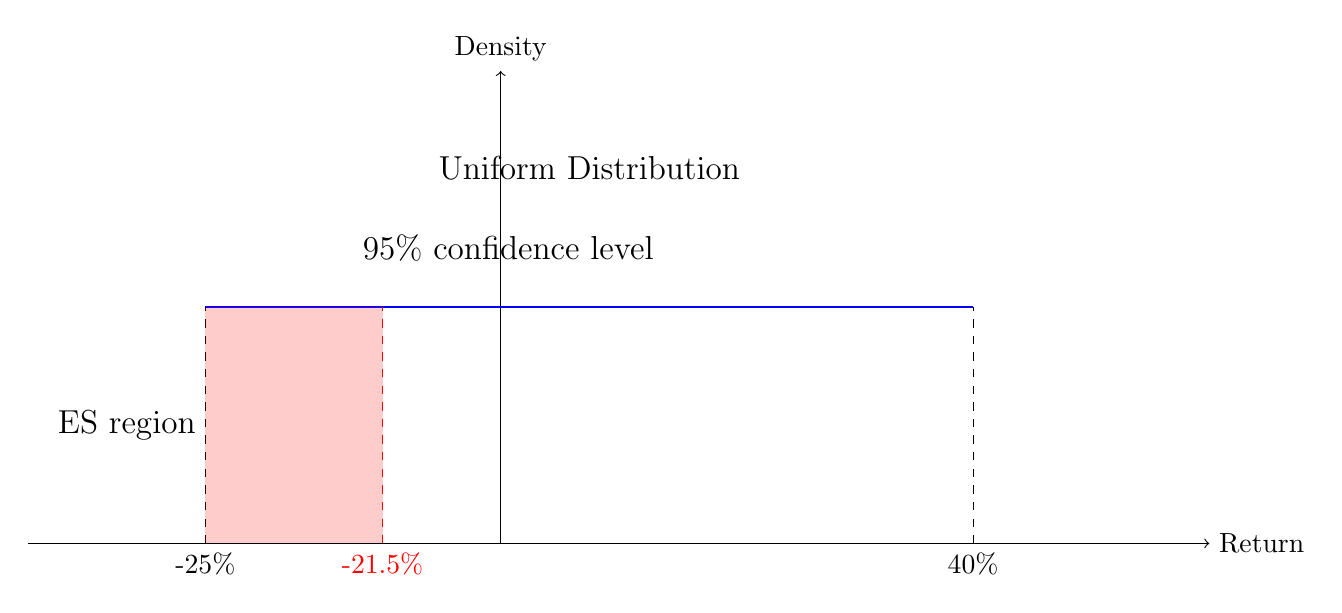
\begin{tikzpicture}[scale=1.5]  % 整体放大1.5倍
                    % 绘制坐标轴
                    \draw[->] (-4,0) -- (6,0) node[right] {Return};
                    \draw[->] (0,0) -- (0,4) node[above] {Density};
                    
                    % 绘制均匀分布的密度函数
                    \draw[thick, blue] (-2.5,2) -- (4,2);
                    \draw[dashed] (-2.5,0) node[below] {-25\%} -- (-2.5,2);
                    \draw[dashed] (4,0) node[below] {40\%} -- (4,2);
                    
                    % 标记VaR
                    \draw[red, dashed] (-1,0) node[below] {-21.5\%} -- (-1,2);
                    
                    % 阴影区域表示ES
                    \fill[red, opacity=0.2] (-2.5,0) -- (-2.5,2) -- (-1,2) -- (-1,0) -- cycle;
                    
                    % 添加标注，字体放大
                    \node[above, font=\large] at (0.75,3) {Uniform Distribution};
                    \node[right, font=\large] at (-1.25,2.5) {95\% confidence level};
                    \node[left, font=\large] at (-2.5,1) {ES region};
                \end{tikzpicture}
                \end{center}
            
            从图中可以看出：
            \begin{itemize}
                \item 蓝线表示均匀分布的概率密度函数
                \item 红色虚线表示95\% VaR的位置（-21.5\%）
                \item 红色阴影区域表示ES计算区间（从-25\%到-21.5\%）
                \item 由于是均匀分布，ES就是阴影区域的平均值（22.75\%）
            \end{itemize}
            
            因此，95\% VaR = 21.5\%，95\% ES = 22.75\%，正确答案为D选项。
            \end{explanation}
            
            \checklist{均匀分布下VaR和ES的计算方法。（图形化理解风险度量）}
    \begin{question}
    In the context of financial risk management, Value at Risk (VaR) is a widely used risk measurement method. A risk management team at a leading financial institution is reviewing the properties and limitations of VaR to ensure its effective application in their investment strategies. During a team meeting, they discuss several statements about VaR. Which of the following statements about VaR is CORRECT?
    \\在金融风险管理背景下，价值风险（VaR）是一种广泛使用的风险度量方法。一家领先金融机构的风险管理团队正在审查VaR的特性和局限性，以确保其在投资策略中的有效应用。在团队会议上，他们讨论了几个关于VaR的陈述。以下哪个陈述关于VaR是正确的？
\end{question}

\begin{choices}
    \item VaR exhibits strong portfolio diversification effects, consistently reflecting the risk reduction benefits when combining multiple investments.\\
    VaR表现出强烈的投资组合多元化效应，持续反映在组合多个投资时的风险降低收益。
    \item VaR provides reliable risk estimates across all market conditions due to its robust statistical foundation in normal distribution theory.\\
    VaR提供了可靠的风险估计，因为它在正态分布理论中具有强大的统计基础。
    \item The standardized confidence levels and holding periods in VaR calculations must be clearly specified and consistently applied to ensure meaningful risk comparisons across portfolios.\\
    VaR计算中的标准化置信水平和持有期必须明确指定并一致应用，以确保投资组合之间的有意义的风险比较。
    \item VaR provides an estimate of the actual amount or size of loss an investor might face, reflecting the corresponding risk exposure.\\
    VaR提供投资者可能面临的实际损失金额或大小的估计，反映相应的风险敞口。
\end{choices}

\begin{correctanswer}
    C
\end{correctanswer}

\begin{explanation}
    \textbf{A选项错误。}
    \begin{itemize}
        \item VaR违反次可加性原则，这意味着当组合多个投资时，组合的VaR可能大于各个投资VaR的总和。这种情况可能导致对整体风险的高估，因为没有考虑到投资组合的多样化效应。
    \end{itemize}

    \textbf{B选项错误。}
    \begin{itemize}
        \item VaR在非正态分布条件下可能不可靠，因为它通常假设收益分布是正态的。在极端事件发生时，VaR可能无法准确捕捉尾部风险，这使得它在处理非正态分布时存在局限性。
    \end{itemize}

    \textbf{C选项正确。}
    \begin{itemize}
        \item VaR的计算确实需要明确指定和一致应用标准化的置信水平和持有期，这是进行有意义的风险比较的基础。例如，不同投资组合之间的VaR比较只有在使用相同的置信水平（如95\%或99\%）和持有期（如1天或10天）时才有意义。
        \item 这种标准化的要求确保了风险度量的可比性和一致性，是VaR作为风险管理工具的重要特征。
    \end{itemize}

    \textbf{D选项错误。}
    \begin{itemize}
        \item VaR并不提供投资者实际损失的金额或大小，它只提供了在给定置信水平下可能的最大损失。相同的VaR值并不意味着风险敞口相同，因为不同的回报分布可能具有相同的VaR，但风险敞口可能非常不同。
    \end{itemize}
\end{explanation}

\checklist{VaR的性质与局限性。（VaR并不提供投资者实际损失的金额或大小）}



\begin{question}
    In the context of financial risk management, understanding the relationship between asset value changes and underlying variables is crucial. A risk management team at a leading financial institution is reviewing the characteristics of linear and nonlinear investment products. During a team meeting, they discuss several statements about these products. Which of the following statements is INCORRECT?
    \\在金融风险管理背景下，理解资产价值变化与基础变量之间的关系至关重要。一家领先金融机构的风险管理团队正在审查线性和非线性投资产品的特性。在团队会议上，他们讨论了几个关于这些产品的陈述。以下哪个陈述是不正确的？
\end{question}

\begin{choices}
    \item The value change of a linear investment portfolio has a linear relationship with the change in its underlying variables. Futures and forwards are typical examples of linear products.\\
    线性投资组合的价值变化与其基础变量的价值变化呈线性关系，期货和远期是线性衍生品的典型例子。
    \item The value change of a nonlinear investment portfolio does not have a linear relationship with the change in its underlying variables. Options are common examples of nonlinear products.\\
    非线性投资组合的价值变化与其基础变量的价值变化没有线性关系，期权是常见的非线性衍生品。
    \item The first derivative of a linear investment portfolio is constant, while the first derivative of a nonlinear investment portfolio is variable.\\
    线性投资组合的一阶导数为常数，非线性投资组合的一阶导数为非常数。
    \item A linear investment portfolio exhibits the same risk sensitivity as a nonlinear investment portfolio during market fluctuations.\\
    线性投资组合在市场波动时不会表现出与非线性投资组合相同的风险敏感度。
\end{choices}

\begin{correctanswer}
    D
\end{correctanswer}

\begin{explanation}
    \textbf{A选项正确。}
    \begin{itemize}
        \item 线性投资组合的价值变化与其基础变量的价值变化呈线性关系，期货和远期是线性衍生品的典型例子。
    \end{itemize}

    \textbf{B选项正确。}
    \begin{itemize}
        \item 非线性投资组合的价值变化与基础变量的价值变化没有线性关系，期权是常见的非线性衍生品。
    \end{itemize}

    \textbf{C选项正确。}
    \begin{itemize}
        \item 线性投资组合的一阶导数为常数，非线性投资组合的一阶导数为非常数。
    \end{itemize}

    \textbf{D选项错误。}
    \begin{itemize}
        \item 线性投资组合在市场波动时不会表现出与非线性投资组合相同的风险敏感度。线性投资组合的风险敏感度通常是可预测的，而非线性投资组合的风险敏感度可能因市场条件的变化而变化，因此它们的风险敏感度不同。
    \end{itemize}
\end{explanation}

\checklist{线性和非线性投资产品的特性与关系。（非线性投资产品的风险敏感度可能因市场条件的变化而变化）}


\begin{question}
    A risk manager is monitoring a domestic equity portfolio valued at USD 100 million using historical VaR with a 100-day lookback period. The initial analysis showed the following extreme negative returns:

    \begin{center}
    \begin{tabular}{|c|c|c|}
    \hline
    Order & Return & Days Ago \\
    \hline
    1 & -10.0\% & 95 \\
    \hline
    2 & -6.3\% & 17 \\
    \hline
    3 & -4.7\% & 65 \\
    \hline
    4 & -4.0\% & 4 \\
    \hline
    5 & -3.8\% & 5 \\
    \hline
    6 & -3.6\% & 30 \\
    \hline
    \end{tabular}
    \end{center}

    Over the next 10 days, four new extreme declines occurred: -25\%, -9.5\%, -7.8\%, and -4.1\%. The other six days showed positive returns. Calculate the updated 1-day 95\% VaR using the historical approach with equal weights.
    \\ 
    一位风险管理经理正在使用历史VaR（100天回顾期）监控一个价值1亿美元的国内股票投资组合。初步分析显示了以下极端负收益：

    \begin{center}
    \begin{tabular}{|c|c|c|}
    \hline
    排序 & 收益率 & 天数前 \\
    \hline
    1 & -10.0\% & 95 \\
    \hline
    2 & -6.3\% & 17 \\
    \hline
    3 & -4.7\% & 65 \\
    \hline
    4 & -4.0\% & 4 \\
    \hline
    5 & -3.8\% & 5 \\
    \hline
    6 & -3.6\% & 30 \\
    \hline
    \end{tabular}
    \end{center}
    在接下来的10天中，发生了四次新的极端下跌：-25\%，-9.5\%，-7.8\%和-4.1\%。其他六天显示正收益。使用等权重历史方法计算更新后的1天95\% VaR。
\end{question}

\begin{choices}
    \item USD 3.28 million\\
    3280000美元
    
    \item USD 4.70 million\\
    4700000美元
    
    \item USD 10.00 million\\
    10000000美元
    
    \item USD 25.00 million\\
    25000000美元
\end{choices}

\begin{correctanswer}
    B
\end{correctanswer}

\begin{explanation}
    \textbf{步骤1：整理更新后的极端损失}
    \begin{itemize}
        \item 按损失从大到小排序：
        \[
        -25.0\%, -9.5\%, -7.8\%, -6.3\%, -4.7\%, -4.1\%
        \]
    \end{itemize}

    \textbf{步骤2：确定VaR位置}
    \begin{itemize}
        \item 总样本量 = 100天
        \[
        \text{95\%分位数位置} = 100 \times 5\% = 5
        \]
        \item 第5个最大损失为4.7\%
    \end{itemize}

    \textbf{步骤3：计算VaR金额}
    \[
    \text{VaR}(95\%) = 4.7\% \times \text{USD 100 million} = \text{USD 4.70 million}
    \]
\end{explanation}

\checklist{历史VaR的更新计算（重点是分位数的确定）}





\fi



\iftrue
\section{考点2:Calculating and Applying VaR}
\setcounter{question}{0}





\begin{question}
    A risk analyst at Bergman International Bank is tasked with explaining how to calculate Value at Risk (VaR) for linear derivatives to new junior analysts. Which of the following statements accurately describes the process for calculating VaR for a linear derivative based on the S\&P 500 Index?
    \\Bergman国际银行的一名风险分析师被要求解释如何计算基于S\&P 500指数的线性衍生品的VaR。以下哪个陈述准确描述了基于S\&P 500指数的线性衍生品的VaR计算过程？
\end{question}

\begin{choices}
    \item For a futures contract, the VaR of the S\&P 500 Index should be multiplied by a sensitivity factor that indicates the percentage change in the futures contract's value for a 1\% change in the index.\\
    对于期货合约，S\&P 500指数的VaR应乘以一个敏感性因子，该因子表示在指数变化1\%时期货合约价值的变化百分比。
    \item For an options contract, the VaR of the S\&P 500 Index should be multiplied by a sensitivity factor that indicates the percentage change in the futures contract's value for a 1\% change in the index.\\
    对于期权合约，S\&P 500指数的VaR应乘以一个敏感性因子，该因子表示在指数变化1\%时期货合约价值的变化百分比。
    \item For a futures contract, the VaR of the S\&P 500 Index should be divided by a sensitivity factor that reflects the absolute change in the futures contract's value for an absolute change in the index.\\
    对于期货合约，S\&P 500指数的VaR应除以一个敏感性因子，该因子表示在指数变化1\%时期货合约价值的变化百分比。
    \item For an options contract, the VaR of the S\&P 500 Index should be divided by a sensitivity factor that indicates the percentage change in the futures contract's value for a 1\% change in the index.\\
    对于期权合约，S\&P 500指数的VaR应除以一个敏感性因子，该因子表示在指数变化1\%时期货合约价值的变化百分比。
\end{choices}

\begin{correctanswer}
    A
\end{correctanswer}


\begin{explanation}
\textbf{A选项正确。}
\begin{itemize}
    \item 对于期货合约，计算VaR时需要将S\&P 500指数的VaR乘以一个敏感性因子（\(|\Delta|\)），该因子反映了在指数价值变化1\%时期货合约价值的变化百分比。这是因为期货合约与基础资产之间的关系是线性的，因此可以通过这种方式调整VaR。
\end{itemize}

\textbf{B选项错误。}
\begin{itemize}
    \item 对于期权合约，VaR的计算不应使用期货合约的敏感性因子。期权的价值变化是非线性的，因此需要使用期权的德尔塔（\(\Delta\)）来进行调整，而不是期货合约的敏感性因子。
\end{itemize}

\textbf{C选项错误。}
\begin{itemize}
    \item 对于期货合约，VaR的计算不应通过除以敏感性因子来进行。相反，应该乘以敏感性因子来反映期货合约的价值变化。
\end{itemize}

\textbf{D选项错误。}
\begin{itemize}
    \item 对于期权合约，VaR的计算同样不应通过除以敏感性因子来进行。期权的价值变化是非线性的，应该使用期权的德尔塔进行调整，而不是期货合约的敏感性因子。
\end{itemize}
\end{explanation}

\checklist{期货合约和期权合约的VaR计算。（区分期权和期货的敏感因子）}







\begin{question}
    A risk manager would like to measure VaR for a bond. He notices that the bond has a 
    puttable feature. What effect on the VaR will this puttable feature have? 
    \\一位风险经理想要测量一个债券的VaR。他注意到债券具有可赎回（puttable）特性。这个可赎回特性对VaR有什么影响？
    \end{question}
    
    \begin{choices}
        \item The VaR will increase.\\
        VaR会增加。
        \item The VaR will decrease.\\
        VaR会减少。
        \item The VaR will remain the same.\\
        VaR会保持不变。
        \item The effect on the VaR will depend on the volatility of the bond.\\
        VaR的影响取决于债券的波动性。
    \end{choices}
    
    \begin{correctanswer}
        B
    \end{correctanswer}

    \begin{explanation}

    \textbf{B选项正确。}

        在这道题中，风险经理注意到债券具有可赎回（puttable）特性。可赎回特性意味着投资者可以在特定条件下将债券“卖回”给发行者。这种特性对VaR（风险价值）的影响如下：
    \begin{itemize}
        \item 可赎回特性意味着投资者拥有一个选择权
        \begin{itemize}
            \item 当债券的市场价格下跌时，投资者可以选择将债券赎回，避免进一步的损失。这就像是投资者拥有一个“保险”，可以在不利情况下保护自己的投资。
        \end{itemize}
    
        \item 正的伽马效应:
            \begin{itemize}
                \item 由于可赎回特性，债券的价格对市场波动的反应会变得更加敏感。这种敏感性被称为“伽马”（\(\Gamma\)）。伽马是期权定价模型中的一个重要参数，表示期权的德尔塔（\(\Delta\)）对基础资产价格变化的敏感度。
                \item 数学上，伽马可以表示为：
                \[
                \Gamma = \frac{\partial^2 C}{\partial S^2}
                \]
                其中，\(C\)是期权的价格，\(S\)是基础资产的价格。正的伽马意味着：
                \[
                \Gamma > 0 \implies \Delta \text{ increases as } S \text{ increases}
                \]
                \item 这意味着当市场价格波动时，债券的价值变化会有更好的保护。具体来说，当市场价格下跌时，投资者可以选择将债券赎回，从而避免更大的损失。这种保护机制降低了潜在的损失，导致VaR（风险价值）降低。
            \end{itemize}
    
        \item VaR的降低:
            \begin{itemize}
                \item 由于投资者可以在不利情况下将债券赎回，这种保护机制会导致VaR降低。换句话说，投资者面临的潜在损失减少了，因此VaR也会相应减少。
            \end{itemize}
    \end{itemize}

    \end{explanation}
\checklist{VaR的计算。（需要知道delta的作用）} 



    \begin{question}
        Two investment banks, Bank X and Bank Y, are calculating the 1-day 99\% VaR for a call option on a non-dividend-paying stock. The relevant information is as follows:
        
        \begin{itemize}
            \item Current stock price: USD 100
            \item Estimated annual volatility: 20\%
            \item Current option price: USD 4.50
            \item Option delta: 0.5
        \end{itemize}
        
        Bank X uses a linear approximation method, while Bank Y employs a Monte Carlo simulation for a more detailed analysis. Which bank is likely to report a higher 1-day 99\% VaR?
        \\两家投资银行，Bank X和Bank Y，正在计算一个非分红股票的看涨期权的1天99\% VaR。相关信息如下：
        \begin{itemize}
            \item 当前股票价格：USD 100
            \item 估计年波动率：20\%
            \item 当前期权价格：USD 4.50
            \item 期权德尔塔：0.5
        \end{itemize}
        Bank X使用线性近似法，而Bank Y使用蒙特卡洛模拟进行更详细的分析。哪一家银行可能报告更高的1天99\% VaR？
    \end{question}
    
    \begin{choices}
        \item Bank X will report a higher VaR.\\ Bank X会报告更高的VaR。  
        \item Bank Y will report a higher VaR.\\ Bank Y会报告更高的VaR。  
        \item Both banks will report the same VaR.\\ 两家银行都会报告相同的VaR。  
        \item Insufficient information to determine.\\ 信息不足，无法确定。  
    \end{choices}
    
    \begin{correctanswer}
        B
    \end{correctanswer}
    
    \begin{explanation}
\textbf{B选项正确。}
\begin{itemize}
    \item 理解计算方法：
    \begin{itemize}
          \item Bank X 使用线性近似法，这种方法通常会低估风险，因为它假设收益是线性的，未能充分考虑潜在的极端情况。
          \item Bank Y 使用蒙特卡洛模拟法，这种方法通过模拟多种市场情景，能够更全面地评估风险，通常会提供更高的VaR估计。
    \end{itemize}
    
        \item 比较两种方法：
        \begin{itemize}
           \item 线性近似法在波动性较高的情况下可能会低估VaR，尤其是在市场波动较大的情况下。
           \item 蒙特卡洛模拟法能够考虑到更复杂的市场动态，因此在大多数情况下会给出更高的VaR估计。
        \end{itemize}
           
    \end{itemize}
    根据上述分析，Bank Y 更有可能估算出更高的1天99\% VaR，因为其方法更为全面和准确。
    \end{explanation}
    
    \checklist{VaR的计算。（VaR和蒙特卡洛模拟的对比）} 



\begin{question}
    A risk analyst at an investment firm is conducting a historical simulation to estimate the Expected Shortfall (ES) of a portfolio. The portfolio's value at market close depends on the stock price and the interest rate. The analyst uses data from the most recent 501 trading days, with Day 0 as the first data point and Day 500 as the last. What stock price and interest rate should the analyst use for Day 501?

    \begin{table}[h]
        \centering
        \begin{tabular}{ccc}
            \hline
            Day & Stock Price (HKD) & Interest Rate (\%) \\
            \hline
            0   & 80.00              & 3.00              \\
            1   & 78.00              & 3.10              \\
            ... & ...                & ...               \\
            500 & 100.00             & 4.00              \\
            \hline
        \end{tabular}
    \end{table}
一位风险分析师正在使用历史模拟法估算一个投资组合的预期短缺（ES）。投资组合的价值在市场收盘时取决于股票价格和利率。分析师使用最近501个交易日的数据，Day 0为第一个数据点，Day 500为最后一个数据点。分析师应该使用哪一天的股票价格和利率来计算Day 501的预期短缺？
\begin{table}[h]
    \centering
    \begin{tabular}{ccc}
        \hline
        天数 & 股价（港元） & 利率（\%） \\
        \hline
        0   & 80.00              & 3.00              \\
        1   & 78.00              & 3.10              \\
        ... & ...                & ...               \\
        500 & 100.00             & 4.00              \\
        \hline
    \end{tabular}
\end{table}

   
\end{question}

\begin{choices}
    \item A. Stock price: HKD 95.00, Interest rate: 4.05\%\\
    股票价格：95.00港元，利率：4.05\%
    \item B. Stock price: HKD 95.00, Interest rate: 4.10\%\\
    股票价格：95.00港元，利率：4.10\%
    \item C. Stock price: HKD 98.00, Interest rate: 4.05\%\\
    股票价格：98.00港元，利率：4.05\%
    \item D. Stock price: HKD 98.00, Interest rate: 4.10\%\\
    股票价格：98.00港元，利率：4.10\%
\end{choices}

\begin{correctanswer}
    B
\end{correctanswer}

\begin{explanation}
    \textbf{步骤1：确定历史变化率}
    \begin{itemize}
        \item 计算从Day 0到Day 1的股票价格变化率：
        \[
        \text{变化率} = \frac{78 - 80}{80} = -0.025 \quad \text{或} \quad -2.5\%
        \]

        \item 计算从Day 0到Day 1的利率变化：
        \[
        \text{变化率} = 3.10\% - 3.00\% = 0.10\%
        \]
    \end{itemize}

    \textbf{步骤2：应用变化率}
    \begin{itemize} 
        \item 将变化率应用于Day 500的股票价格和利率：
        
        \item 股票价格的计算：
        \[
        \text{新股票价格} = 100 \times (1 - 0.025) =  97.50 \quad \text{(约为 HKD 97.50)}
        \]

        \item 利率的计算：
        \[
        \text{新利率} = 4.00\% + 0.10\% = 4.10\%
        \]
    \end{itemize}

\end{explanation}

\checklist{历史模拟法。（根据历史数据计算股票价格和利率的变化）} 





\begin{question}
    A risk management team is discussing different approaches to value at risk (VaR) estimation. Which of the following statements about VaR estimation methods is CORRECT?
    \\一个风险管理团队正在讨论不同的价值风险（VaR）估计方法。以下哪个陈述关于VaR估计方法是正确的？
\end{question}

\begin{choices}
    \item Parametric VaR approaches are primarily forward-looking and rely minimally on historical return data for parameter estimation.\\
    参数法VaR主要是前瞻性的，最小依赖于历史收益率数据来估计参数。
    
    \item GARCH(1,1) models can generate accurate VaR estimates without requiring any historical volatility or return information.\\
    GARCH(1,1)模型可以生成准确的VaR估计，不需要任何历史波动率或收益率信息。
    
    \item Hybrid approaches combining parametric and nonparametric methods are completely independent of historical market data.\\
    混合方法结合了参数法和非参数法的特点，完全独立于历史市场数据。
    
    \item Implied volatility-based VaR estimation is the least dependent on historical returns as it primarily uses current option market prices.\\
    隐含波动率法VaR估计对历史收益率的依赖最小，因为它主要使用当前期权市场价格。
\end{choices}

\begin{correctanswer}
    D
\end{correctanswer}

\begin{explanation}
    \textbf{A选项错误。} 
    \begin{itemize}
        \item 参数法VaR高度依赖历史数据，因为需要使用历史收益率来估计均值、波动率等参数。这些参数的准确性直接影响VaR的计算结果。
    \end{itemize}

    \textbf{B选项错误。} 
    \begin{itemize}
        \item GARCH(1,1)模型本质上是一个基于历史数据的模型，需要历史收益率序列来估计波动率持续性参数，其预测能力取决于历史数据的质量。
    \end{itemize}

    \textbf{C选项错误。} 
    \begin{itemize}
        \item 混合方法结合了参数法和非参数法的特点，其中非参数部分直接使用历史数据，参数部分也需要历史数据来估计参数，因此无法完全独立于历史市场数据。
    \end{itemize}

    \textbf{D选项正确。} 
    \begin{itemize}
        \item 隐含波动率方法主要使用当前期权市场价格，反映了市场对未来波动率的预期，相比其他方法，对历史收益率数据的依赖最小。这种方法更多地体现了市场的前瞻性预期。
    \end{itemize}
\end{explanation}
\checklist{VaR估计方法比较（重点是各种方法对历史数据的依赖程度）}



\begin{question}
    A bank's operational risk department has developed a model for a specific business process. For the next year, the model predicts a 95\% probability of no loss occurrence and a 5\% probability of experiencing a loss event. If a loss occurs, there are three possible outcomes: a \$12 million loss with 20\% probability, a \$20 million loss with 50\% probability, and a \$28 million loss with 30\% probability. What is the 90\% Expected Shortfall (ES) for this operational risk model?
    \\一家银行的操作风险部门开发了一个特定业务流程的模型。明年，模型预测95\%的概率没有损失发生，5\%的概率发生损失事件。如果发生损失，有三种可能的结果：1200万美元损失的概率为20\%，2000万美元损失的概率为50\%，2800万美元损失的概率为30\%。这个操作风险模型的90\%预期短缺（ES）是多少？
\end{question}

\begin{choices}
    \item \$10.4 million\\
    1040万美元
    
    \item \$12.0 million\\
    1200万美元
    
    \item \$15.6 million\\
    1560万美元
    
    \item \$20.0 million\\
    2000万美元
\end{choices}

\begin{correctanswer}
    A
\end{correctanswer}

\begin{explanation}
    \textbf{步骤1：理解90\%ES的计算范围。}
        \[
        \text{10\%尾部 = 无损失区间(90\%-95\%, 占5\%) + 损失事件区间(95\%-100\%, 占5\%)}
        \]

    \textbf{步骤2：计算损失事件的条件期望值。}
        \[
        E(\text{损失}|\text{损失发生}) = \sum_{i=1}^{3} p_i \times L_i
        \]
        \[
        = 20\% \times \$12M + 50\% \times \$20M + 30\% \times \$28M
        \]
        \[
        = \$2.4M + \$10.0M + \$8.4M = \$20.8M
        \]

    \textbf{步骤3：计算90\% ES。}
        \[
        \text{ES}_{90\%} = \frac{\text{无损失部分} + \text{损失部分}}{10\%}
        \]
        \[
        = \frac{5\% \times \$0 + 5\% \times \$20.8M}{10\%}
        \]
        \[
        = \frac{\$0 + \$1.04M}{10\%} = \$10.4M
        \]
\end{explanation}

\checklist{操作风险的ES计算（重点是条件期望和分布组合）}


\begin{question}
    A portfolio manager is reviewing the effectiveness of diversification strategies during the 2008 financial crisis. The analysis focuses on how correlations between different asset classes changed during this period and its implications for risk management. Which of the following statements MOST accurately describes the behavior of correlations and risk metrics during financial crises?
    \\一位投资组合经理正在审查2008年金融危机期间多元化策略的有效性。分析重点是不同资产类别之间的相关性在危机期间如何变化及其对风险管理的影响。以下哪个陈述最准确地描述了金融危机期间相关性和风险度量行为？
\end{question}

\begin{choices}
    \item Historical correlations between asset classes remain stable during crisis periods, making traditional diversification strategies consistently effective.\\
    资产类别之间的历史相关性在危机期间保持稳定，使传统多元化策略始终有效。
    
    \item Asset correlations tend to increase significantly during market stress, reducing diversification benefits and leading to higher portfolio risk levels.\\
    资产相关性在市场压力期间倾向于显著增加，降低多元化收益并导致更高的投资组合风险水平。
    
    \item Market volatilities increase during crises but correlations typically decrease, creating new diversification opportunities.\\
    市场波动率在危机期间增加，但相关性通常下降，创造了新的多元化机会。
    
    \item Standard VaR models automatically adjust for changing correlations during crisis periods, making additional risk adjustments unnecessary.\\
    标准VaR模型在危机期间自动调整相关性变化，使额外风险调整不必要。
\end{choices}

\begin{correctanswer}
    B
\end{correctanswer}

\begin{explanation}
    \textbf{A选项错误。} 
    \begin{itemize}
        \item 这与经验证据相反。研究表明，金融危机期间资产间的相关性会发生显著变化，传统的多元化策略效果会减弱。
    \end{itemize}

    \textbf{B选项正确。} 
    \begin{itemize}
        \item 这反映了"相关性趋同"(correlation convergence)现象：危机期间，大多数资产类别之间的相关性会显著上升；这种相关性增加降低了投资组合多元化的效果，导致在最需要分散化保护时，其效果反而最差。
    \end{itemize}

    \textbf{C选项错误。} 
    \begin{itemize}
        \item 这与实际观察相反。危机期间，不仅波动率上升，相关性也会上升，这实际上减少了而不是创造了多元化机会。
    \end{itemize}

    \textbf{D选项错误。} 
    \begin{itemize}
        \item 标准VaR模型通常使用历史数据估计相关性，无法及时反映危机期间的相关性突变，这正是为什么需要补充使用压力测试等其他风险管理工具。
    \end{itemize}
\end{explanation}

\checklist{金融危机期间的相关性变化（重点是相关性趋同现象及其对风险管理的影响）}


\begin{question}
    A risk analyst is evaluating the risk metrics for a trading portfolio using historical simulation. The following 25 ordered percentage returns have been generated:

    -18, -15, -12, -10, -8, -6, -5, -5, -3, -2, -1, 0, 0, 1, 2, 3, 5, 7, 8, 10, 12, 15, 17, 20, 22

    Required:
    (1) Calculate the Value at Risk (VaR) at 90\% confidence level
    (2) Calculate the Expected Shortfall (ES) at 90\% confidence level
    \\一位风险分析师正在使用历史模拟法评估一个交易组合的风险度量。以下25个排序后的百分比收益已被生成：
    -18, -15, -12, -10, -8, -6, -5, -5, -3, -2, -1, 0, 0, 1, 2, 3, 5, 7, 8, 10, 12, 15, 17, 20, 22
    要求：
    (1) 计算90\%置信水平下的价值风险（VaR）
    (2) 计算90\%置信水平下的预期短缺（ES）
\end{question}

\begin{choices}
    \item VaR(90\%) = 8\%, ES = 11\%\\
    90\%置信水平下的价值风险为8\%，预期短缺为11\%
    
    \item VaR(90\%) = 12\%, ES = 15\%\\
    90\%置信水平下的价值风险为12\%，预期短缺为15\%
    
    \item VaR(90\%) = 12\%, ES = 13.5\%\\
    90\%置信水平下的价值风险为12\%，预期短缺为13.5\%
    
    \item VaR(90\%) = 15\%, ES = 18\%\\
    90\%置信水平下的价值风险为15\%，预期短缺为18\%
\end{choices}

\begin{correctanswer}
    C
\end{correctanswer}

\begin{explanation}
    \textbf{步骤1：计算90\% VaR。}
    \begin{itemize}
        \item 对于n = 25个观察值，确定分位数位置：
        \[
        \text{位置} = n \times (1-90\%) = 25 \times 10\% = 2.5
        \]
        \item 取第3个最低值：-12\%
        \[
        \text{VaR}(90\%) = |-12\%| = 12\%
        \]
    \end{itemize}

    \textbf{步骤2：计算90\% ES。}
    \begin{itemize}
        \item 计算VaR以外损失的平均值：
        \[
        \text{ES}(90\%) = \frac{|-18\%| + |-15\%|}{2} = \frac{33\%}{2} = 13.5\%
        \]
    \end{itemize}

    \textbf{结论：} VaR(90\%) = 12\%, ES(90\%) = 13.5\%
\end{explanation}

\checklist{VaR和ES的历史模拟计算（重点是分位数确定和条件期望计算）}



\begin{question}
    A risk manager at a global fund believes that the market is about to transition from a bull to a bear market. She needs to select appropriate risk measures and calculation methods to assess the portfolio's risk exposure during this transition period. Which of the following statements is CORRECT regarding the choice and implementation of risk measures?
    \\一位全球基金的风险经理认为市场即将从牛市转为熊市。她需要选择适当的风险度量和计算方法来评估投资组合在转型期间的风险暴露。以下哪个陈述关于风险度量和计算方法的选择和实施是正确的？
\end{question}

\begin{choices}
    \item VaR and Expected Shortfall are equivalent in measuring tail risk, as both metrics capture the complete distribution of potential losses in the portfolio's tail.\\
    VaR和预期短缺在衡量尾部风险方面是等价的，因为两者都捕捉了投资组合尾部潜在损失的完整分布。
    
    \item Historical simulation remains a reliable method for VaR calculation during market regime changes, as past price patterns and correlations will continue to be representative.\\
    历史模拟在市场机制变化期间仍然是计算VaR的可靠方法，因为过去的价格模式和相关性将继续具有代表性。
    
    \item Monte Carlo simulation with appropriate distributional assumptions and volatility adjustments is suitable for VaR calculation during market transitions, as it allows for flexible modeling of changing market conditions.\\
    蒙特卡洛模拟，具有适当的分布假设和波动率调整，适合在市场转型期间计算VaR，因为它允许灵活建模市场条件的变化。
    
    \item For portfolios containing options, the delta-normal approach without gamma adjustment provides accurate VaR estimates, as option risks are primarily linear in nature.\\
    对于包含期权的投资组合，delta-normal方法不进行gamma调整提供准确的VaR估计，因为期权风险主要是线性的。
\end{choices}

\begin{correctanswer}
    C
\end{correctanswer}

\begin{explanation}
    \textbf{A选项错误。} 
    \begin{itemize}
        \item VaR只衡量特定分位点的损失，而ES才能完整描述尾部风险分布。两者在尾部风险刻画能力上存在本质差异。
    \end{itemize}

    \textbf{B选项错误。} 
    \begin{itemize}
        \item 市场转型期间，历史数据的代表性显著下降。历史模拟方法过度依赖过去数据，无法准确反映市场机制的根本变化。
    \end{itemize}

    \textbf{C选项正确。} 
    \begin{itemize}
        \item 蒙特卡洛模拟允许灵活调整波动率和相关性假设，可以通过参数调整反映市场状态转换，适合建模转型期间的风险特征。
    \end{itemize}

    \textbf{D选项错误。} 
    \begin{itemize}
        \item 期权具有显著的非线性特征，忽略gamma效应会严重低估风险。在市场剧烈波动时期，这种低估会更加严重。
    \end{itemize}
\end{explanation}

\checklist{风险度量方法选择（重点是不同方法在市场转型期的适用性）}


\begin{question}
    A portfolio manager at a university endowment fund is comparing different VaR calculation methods for their €80,000,000 equity portfolio. The portfolio has the following characteristics:

    \begin{itemize}
        \item Daily expected return: 0.05\%
        \item Daily volatility: 0.85\%
        \item Significance level: 2\% (z-value = 2.05)
    \end{itemize}

    The manager also collected 250 daily historical returns. The six lowest returns are:
    \begin{center}
    \begin{tabular}{|c|c|}
    \hline
    Rank & Return \\
    \hline
    1 & -3.25\% \\
    \hline
    2 & -2.88\% \\
    \hline
    3 & -2.65\% \\
    \hline
    4 & -2.42\% \\
    \hline
    5 & -2.28\% \\
    \hline
    6 & -2.15\% \\
    \hline
    \end{tabular}
    \end{center}

    Compare the daily VaR estimates using both delta-normal and historical simulation methods.
    \\一位大学捐赠基金的投资组合经理正在比较其8000万欧元股票投资组合的不同VaR计算方法。该投资组合具有以下特征：

    \begin{itemize}
        \item 每日预期收益率：0.05\%
        \item 每日波动率：0.85\%
        \item 显著性水平：2\%（z值 = 2.05）
    \end{itemize}

    该经理还收集了250个每日历史收益率。六个最低收益率如下：
    \begin{center}
    \begin{tabular}{|c|c|}
    \hline
    排名 & 收益率 \\
    \hline
    1 & -3.25\% \\
    \hline
    2 & -2.88\% \\
    \hline
    3 & -2.65\% \\
    \hline
    4 & -2.42\% \\
    \hline
    5 & -2.28\% \\
    \hline
    6 & -2.15\% \\
    \hline
    \end{tabular}
    \end{center}

    使用delta-normal方法和历史模拟方法比较每日VaR估计值。
\end{question}

\begin{choices}
    \item Both methods give the same VaR estimate of €2.12 million\\
    两种方法都给出2120万欧元的VaR估计值
    
    \item Delta-normal: €1.68 million; Historical: €2.12 million\\
    Delta-normal: 1680万欧元；历史模拟: 2120万欧元
    
    \item Delta-normal: €1.32 million; Historical: €1.82 million\\
    Delta-normal: 1320万欧元；历史模拟: 1820万欧元
    
    \item Delta-normal: €2.12 million; Historical: €1.68 million\\
    Delta-normal: 2120万欧元；历史模拟: 1680万欧元
\end{choices}

\begin{correctanswer}
    B
\end{correctanswer}

\begin{explanation}
    \textbf{步骤1：计算Delta-normal VaR}
    \[
    \text{VaR}_{\text{Delta-normal}} = [-(\mu - z\sigma)] \times \text{Portfolio Value}
    \]
    \[
    = [-(0.05\% - 2.05 \times 0.85\%)] \times €80,000,000
    \]
    \[
    = [0.05\% + 1.74\%] \times €80,000,000 = €1.68 \text{ million}
    \]

    \textbf{步骤2：计算Historical VaR}
    \[
    \text{观察数} = 250, \text{分位点} = 250 \times 2\% = 5
    \]
    \[
    \text{第5个最低收益率} = -2.65\%
    \]
    \[
    \text{VaR}_{\text{Historical}} = 2.65\% \times €80,000,000 = €2.12 \text{ million}
    \]
\end{explanation}

\checklist{VaR计算方法比较（参数法vs历史模拟法）}


\begin{question}
    A junior risk analyst at an asset management firm is currently evaluating different methods for assessing portfolio risk. The analyst is particularly interested in historical simulation due to its straightforward approach and reliance on past data. During a team meeting, the analyst presents several statements about historical simulation to discuss its advantages and limitations. Which of the following statements about historical simulation is correct?
    \\一位资产管理部门的初级风险分析师正在评估不同的风险评估方法。分析师特别关注历史模拟，因为它简单直接且依赖于过去的数据。在团队会议上，分析师提出了几个关于历史模拟的陈述，讨论其优势和局限性。以下哪个陈述关于历史模拟是正确的？
\end{question}

\begin{choices}
    \item Historical simulation provides dynamic updates to volatility and correlation estimates through continuous market feedback mechanisms.\\
    历史模拟通过连续的市场反馈机制动态更新波动率和相关性估计。
    
    \item Historical simulation incorporates time-varying weights to reflect the relative importance of recent versus distant observations.\\
    历史模拟采用时间可变权重来反映近期观察与远期观察的相对重要性。
    
    \item Historical simulation does not require any model assumptions.\\
    历史模拟不需要任何模型假设。
    
    \item Historical simulation generates reliable future market predictions through comprehensive pattern recognition algorithms.\\
    历史模拟通过综合模式识别算法生成可靠的未来市场预测。
\end{choices}

\begin{correctanswer}
    C
\end{correctanswer}

\begin{explanation}
    \textbf{A选项错误。}
    \begin{itemize}
        \item 历史模拟法是一种静态方法，它不能动态更新波动率和相关性估计。它仅仅使用历史数据进行模拟，无法通过市场反馈机制来更新估计值。
    \end{itemize}

    \textbf{B选项错误。}
    \begin{itemize}
        \item 标准历史模拟法对所有观察值赋予相同的权重，并不会根据观察值的时间远近来调整权重。这种平等权重的特性可能会导致无法充分反映最近市场变化的影响。
    \end{itemize}

    \textbf{C选项正确。}
    \begin{itemize}
        \item 历史模拟法作为一种非参数方法，确实不需要依赖任何特定的模型假设。它直接使用历史数据来生成可能的市场情景，这是其主要优势之一。
    \end{itemize}

    \textbf{D选项错误。}
    \begin{itemize}
        \item 历史模拟法并不包含模式识别算法，它仅仅基于历史数据进行简单的重采样。它不能保证对未来市场行为做出可靠预测，因为历史模式可能不会在未来重复。
    \end{itemize}
\end{explanation}

\checklist{历史模拟法的特征（作为一种非参数方法的优势）}


\begin{question}
    A junior risk analyst at an investment firm is evaluating the delta-normal method for risk assessment. The analyst presents several statements about the delta-normal method during a team meeting. Which of the following statements is CORRECT?
    \\一位投资公司的初级风险分析师正在评估delta-normal方法的风险评估。分析师在团队会议上提出了几个关于delta-normal方法的陈述。以下哪个陈述是正确的？
\end{question}

\begin{choices}
    \item The delta-normal method performs well for linear portfolios and can be applied to nonlinear portfolios.\\
    Delta-normal方法对线性投资组合表现良好，可以应用于非线性投资组合。
    \item The delta-normal method primarily relies on historical volatility patterns to determine the distribution of portfolio returns.\\
    Delta-normal方法主要依赖历史波动模式来确定投资组合收益的分布。
    \item In the delta-normal method, actual changes in all risk factors are more practical than percentage changes.\\
    Delta-normal方法中，所有风险因素的实际变化比百分比变化更实用。
    \item The delta-normal method achieves optimal results through dynamic correlation adjustments in varying market conditions.\\
    Delta-normal方法通过在不同市场条件下进行动态相关性调整实现最佳结果。
\end{choices}

\begin{correctanswer}
    A
\end{correctanswer}

\begin{explanation}
    \textbf{A选项正确。}
    \begin{itemize}
        \item Delta-normal 方法确实适用于线性依赖于市场变量的投资组合，并且在处理这类投资组合时表现良好。此外，虽然它主要用于线性投资组合，但也可以通过近似方法用于非线性投资组合。（教材的观点是可以用在非线性投资组合上，但是只是个近似值，倒不是说不能用。）
    \end{itemize}

    \textbf{B选项错误。}
    \begin{itemize}
        \item Delta-normal 方法主要基于正态分布假设，而不是依赖历史波动率模式。它假设投资组合价值的变化服从正态分布，这是一个前提假设，而不是通过历史数据得出的结论。
    \end{itemize}

    \textbf{C选项错误。}
    \begin{itemize}
        \item Delta-normal 方法并不是对所有风险因素都假设实际变化比百分比变化更实用。实际上，风险因素的适用性取决于具体情况：
        \begin{itemize}
            \item 对于股票和商品价格等风险因素，百分比变化可能更实用。
            \item 对于利率和信用利差等风险因素，实际变化可能更实用。
        \end{itemize}
        因此，不能一概而论地说所有风险因素的实际变化都比百分比变化更实用。
    \end{itemize}

    \textbf{D选项错误。}
    \begin{itemize}
        \item Delta-normal 方法使用固定的相关性假设，并不会动态调整相关性。它假设相关性在计算期间保持稳定，这实际上是该方法的一个局限性，而不是优势。
    \end{itemize}
\end{explanation}

\checklist{Delta-normal方法的局限性（它主要用于线性投资组合，但也可以通过近似方法用于非线性投资组合）}

\begin{question}
    Consider a portfolio consisting of a \$10,000 investment in asset X and a \$20,000 investment in asset Y. Assume the daily volatilities of X and Y are 1\% and 2\% respectively, and the correlation coefficient between their returns is 0.3. Which of the following options correctly describes the portfolio's five-day VaR and ES at a 97\% confidence level?
    \\考虑一个投资组合，包含10,000美元的资产X投资和20,000美元的资产Y投资。假设资产X和Y的每日波动率分别为1\%和2\%，它们之间的相关系数为0.3。以下哪个选项正确描述了该投资组合五天VaR和ES在97\%置信水平下的值？
\end{question}

\begin{choices}
    \item VaR is \$1852.4, ES is \$2233.8.\\
    VaR是1852.4美元，ES是2233.8美元。
    \item VaR is \$2233.8, ES is \$1852.4.\\
    VaR是2233.8美元，ES是1852.4美元。
    \item VaR is \$440.5, ES is \$984.9.\\
    VaR是440.5美元，ES是984.9美元。
    \item VaR is \$984.9, ES is \$440.5.\\
    VaR是984.9美元，ES是440.5美元。
\end{choices}

\begin{correctanswer}
    A
\end{correctanswer}

\begin{explanation}
    \textbf{理论公式：}
    \[
    \text{VaR} = \mu_P - z\sigma_P
    \]
    \[
    \text{ES} = \mu_P + \sigma_P \frac{e^{-(z^2/2)}}{(1-x)\sqrt{2\pi}}
    \]
    其中，\(x\) 是置信水平，\(z\) 是正态分布中超过该概率的点。

    \textbf{步骤1：计算投资组合的日变化标准差}
    \begin{itemize}
        \item \(\sigma_P = \sqrt{100^2 + 400^2 + 2 \times 100 \times 400 \times 0.3} = 440.5\)
    \end{itemize}

    \textbf{步骤2：计算五天变化的标准差}
    \begin{itemize}
        \item \(\sigma_{5P} = \sqrt{5} \times 440.5 = 984.9\)
    \end{itemize}

    \textbf{步骤3：计算五天 VaR（97\% 置信水平）}
    \begin{itemize}
        \item \(\text{VaR}_{5P} = 1.88 \times 984.9 = 1852.4\)
    \end{itemize}

    \textbf{步骤4：计算五天 ES（97\% 置信水平）}
    \begin{itemize}
        \item \(\text{ES}_{5P} = 984.9 \frac{e^{-1.88^2/2}}{0.03\sqrt{2\pi}} = 2233.8\)
    \end{itemize}
\end{explanation}

\checklist{VaR和ES计算（重点是使用Delta-normal方法进行计算）}


\begin{question}
    A quantitative analyst at a global investment bank is evaluating different VaR calculation methods for their complex derivatives portfolio. During a team discussion about Monte Carlo simulation, which of the following statements about this method is CORRECT?
    \\一位全球投资银行的量化分析师正在评估不同的VaR计算方法用于其复杂的衍生品投资组合。在团队讨论蒙特卡洛模拟时，以下哪个陈述关于这种方法是正确的？
\end{question}

\begin{choices}
    \item The Monte Carlo simulation primarily relies on historical data patterns, making it more reliable than parametric approaches for risk factor distribution estimation.\\
    Monte-Carlo模拟主要依赖历史数据模式，使其在风险因子分布估计方面比参数法更可靠。
    \item The Monte Carlo simulation's model risk can be effectively eliminated by increasing the number of simulations and using more sophisticated probability distributions.\\
    Monte-Carlo模拟的模型风险可以通过增加模拟次数和使用更复杂的概率分布有效地消除。
    \item The Monte Carlo simulation is computationally intensive, making it suitable for scenarios requiring quick results.\\
    Monte-Carlo模拟计算量大，适用于需要快速结果的场景。
    \item Using historical data to estimate risk factor characteristics may not accurately predict future market changes.\\
    使用历史数据估计风险因子特性可能无法准确预测未来市场变化。
\end{choices}

\begin{correctanswer}
    D
\end{correctanswer}

\begin{explanation}
    \textbf{A选项错误。}
    \begin{itemize}
        \item 蒙特卡洛模拟并不主要依赖历史数据模式，而是通过假设风险因子的概率分布来生成随机样本。虽然历史数据可以用来估计分布参数，但模拟的核心是基于概率分布的随机抽样过程。
    \end{itemize}

    \textbf{B选项错误。}
    \begin{itemize}
        \item 增加模拟次数和使用更复杂的概率分布可以改善模拟结果，但不能完全消除模型风险。模型风险源于对市场行为的基本假设，这种风险无法仅通过技术改进来消除。
    \end{itemize}

    \textbf{C选项错误。}
    \begin{itemize}
        \item 蒙特卡洛模拟法计算量大，适用于需要详细结果的场景，而不是快速结果。由于需要生成大量的随机样本来进行模拟，蒙特卡洛模拟通常需要较长的计算时间，因此不适合需要快速结果的场景。
    \end{itemize}

    \textbf{D选项正确。}
    \begin{itemize}
        \item 使用历史数据估计风险因子的特性，未必能准确预测未来市场变化。历史数据反映的是过去的市场行为，而未来市场可能会受到不同因素的影响，因此仅依赖历史数据可能无法准确预测未来的市场变化。
    \end{itemize}
\end{explanation}

\checklist{蒙特卡洛模拟法的局限性（计算量大，不适合快速结果）}


\begin{question}
    A risk manager at a global investment bank is evaluating different VaR calculation methods for their diverse portfolio. During their analysis, they notice that each method has its own strengths and limitations in capturing different types of risks. After reviewing the characteristics of Delta-Normal, Historical Simulation, and Monte Carlo Simulation methods, which of the following statements about these approaches is CORRECT?
    \\一位全球投资银行的风险经理正在评估不同的VaR计算方法用于其多样化的投资组合。在分析过程中，他们注意到每种方法在捕捉不同类型风险方面都有其优势和局限性。在审查Delta-Normal、历史模拟和蒙特卡洛模拟方法的特征后，以下哪个陈述关于这些方法的正确？
\end{question}

\begin{choices}
    \item The Delta-Normal method provides comprehensive risk assessment for option portfolios through its linear approximation approach, making it particularly suitable for complex derivatives.\\
    Delta-Normal方法通过其线性近似方法为期权投资组合提供全面的风险评估，使其特别适用于复杂衍生品。
    
    \item The Historical Simulation method maintains consistent computational efficiency across all portfolio types, with enhanced accuracy for structured products.\\
    历史模拟方法在所有投资组合类型中保持一致的计算效率，对结构化产品具有增强的准确性。
    
    \item The Monte Carlo Simulation method is computationally complex but can achieve good VaR precision through multiple iterations.\\
    Monte-Carlo模拟方法计算复杂，但可以通过多次迭代实现良好的VaR精度。
    
    \item The Delta-Normal method performs excellently in VaR precision over short windows, while the Historical Simulation method has advantages in handling time-varying risks and unusual events.\\
    Delta-Normal方法在短期窗口期的VaR精度方面表现出色，而历史模拟方法在处理时变风险和异常事件方面具有优势。
\end{choices}

\begin{correctanswer}
    C
\end{correctanswer}

\begin{explanation}
    \textbf{A选项错误。}
    \begin{itemize}
        \item Delta-Normal方法虽然计算简单，但其线性近似方法在处理期权等非线性产品时存在明显局限性。它可能会低估非线性产品的风险，特别是在处理复杂衍生品时的高值概率估计不准确。
    \end{itemize}

    \textbf{B选项错误。}
    \begin{itemize}
        \item 历史模拟法的计算效率实际上会随着投资组合复杂度增加而降低，对于结构化产品尤其如此。此外，其准确性很大程度上依赖于历史数据的代表性。
    \end{itemize}

    \textbf{C选项正确。}
    \begin{itemize}
        \item 蒙特卡洛模拟法确实计算复杂，需要大量的计算资源，但通过增加模拟次数，可以提高VaR计算的精度。这种通过迭代提高精度的特性是该方法的重要优势。
    \end{itemize}

    \textbf{D选项错误。}
    \begin{itemize}
        \item Delta-Normal方法在短窗口期的VaR精度并不一定优于其他方法，尤其是在处理非线性风险时。历史模拟法在处理时间变化风险和不寻常事件时确实具有优势，但 Delta-Normal方法在这方面并不突出。
    \end{itemize}
\end{explanation}

\checklist{历史模拟法、蒙特卡洛模拟法和Delta-Normal三种方法的比较（综合起来考察）}
\begin{question}
    A junior risk analyst at an asset management firm is currently evaluating different methods for assessing portfolio risk. The analyst is particularly interested in historical simulation due to its straightforward approach and reliance on past data. During a team meeting, the analyst presents several statements about historical simulation to discuss its advantages and limitations. Which of the following statements about historical simulation is CORRECT?
    \\一位资产管理部门的初级风险分析师正在评估不同的风险评估方法。分析师特别关注历史模拟，因为它简单直接且依赖于过去的数据。在团队会议上，分析师提出了几个关于历史模拟的陈述，讨论其优势和局限性。以下哪个陈述关于历史模拟是正确的？
\end{question}

\begin{choices}
    \item Worst Case Analysis primarily serves as a predictive tool for future market movements, providing reliable forecasts through statistical extrapolation of historical extreme events.\\
    最坏情况分析主要是作为预测未来市场走势的工具，通过统计外推历史极端事件提供可靠的预测。
    
    \item Contagion effects occur when both volatility and correlation increase, enhancing the benefits of diversification. VaR and ES can be used to simulate this effect.\\
    传染效应发生在波动率和相关性都增加时，增强分散化的好处。VaR和ES可以用于模拟这种效应。
    
    \item Correlation patterns maintain stability across different market conditions, allowing for consistent risk estimation regardless of market stress levels.\\
    相关性模式在不同市场条件下保持稳定，允许在不同市场压力水平下进行一致的风险估计。
    
    \item When calculating VaR or ES, we should estimate correlations under extreme market conditions rather than normal market conditions.\\
    在计算VaR或ES时，我们应该估计极端市场条件下的相关性，而不是正常市场条件下的相关性。
\end{choices}

\begin{correctanswer}
    D
\end{correctanswer}

\begin{explanation}
    \textbf{A选项错误。}
    \begin{itemize}
        \item 最坏情况分析主要是作为VaR的补充措施，用于理解历史极端损失的分布特征，而不是预测未来市场走势。它的主要功能是帮助理解潜在风险暴露，而不是提供可靠的未来预测。
    \end{itemize}

    \textbf{B选项错误。}
    \begin{itemize}
        \item 传染效应通常在波动率和相关性都增加时发生，这会抵消任何分散化的好处，而不是增强分散化的好处。VaR和ES可以用于模拟危机事件中可能发生的传染效应。
    \end{itemize}

    \textbf{C选项错误。}
    \begin{itemize}
        \item 相关性模式在不同市场条件下并不稳定。特别是在压力市场条件下，相关性通常会显著增加，这种现象被称为相关性崩溃，会导致传统的风险估计方法失效。
    \end{itemize}

    \textbf{D选项正确。}
    \begin{itemize}
        \item 在计算VaR或ES时，我们应该估计极端市场条件下的相关性，而不是正常市场条件下的相关性。这是因为在极端市场条件下，相关性可能会显著变化。
    \end{itemize}
\end{explanation}
\checklist{压力环境的情况（传染效应会抵消分散效应）}




\fi


\iftrue
\section{考点3:Measuring and Monitoring Volatility}
\setcounter{question}{0}






\begin{question}
    A financial analyst is evaluating different models for estimating the volatility of asset returns in order to improve risk management strategies. The analyst comes across four statements regarding these models. Which of the following statements is INCORRECT?
    \\一位金融分析师正在评估不同的模型来估计资产收益率的波动率，以改进风险管理策略。分析师遇到了关于这些模型的四个陈述。以下哪个陈述是不正确的？
\end{question}

\begin{choices}
    \item In the exponentially weighted moving average (EWMA) model, some positive weight is assigned to the long-run average variance.\\
    在指数加权移动平均（EWMA）模型中，分配给长期平均方差的一些正权重。
    \item In the EWMA model, the weights assigned to observations decrease exponentially as the observations become older.\\
    在EWMA模型中，分配给观察值的权重随着观察值变得更旧而指数递减。
    \item In the GARCH (1,1) model, a positive weight is estimated for the long-run average variance.\\
    在GARCH (1,1)模型中，为长期平均方差估计了一个正权重。
    \item In the GARCH (1,1) model, the weights estimated for observations decrease exponentially as the observations become older.\\
    在GARCH (1,1)模型中，估计的观察值的权重随着观察值变得更旧而指数递减。
\end{choices}

\begin{correctanswer}
    A
\end{correctanswer}

\begin{explanation}
    \textbf{A选项错误。} 
    \begin{itemize}
        \item 在EWMA模型中，更新波动率时并不涉及长期平均方差。换句话说，分配给长期平均方差的权重为零。公式为：
        \[
        \sigma_t^2 = (1 - \lambda) \sum_{i=0}^{t-1} \lambda^i r_{t-i}^2
        \]
        其中，\(\lambda\) 是衰减因子，长期平均方差不参与计算。
    \end{itemize}
    
    \textbf{B选项正确。} 
    \begin{itemize}
        \item 在EWMA模型中，分配给观察值的权重确实是随着观察值变得更旧而指数递减的。公式为：
        \[
        w_i = \lambda^i
        \]
        这表明较新的观察值对波动率的影响更大。
    \end{itemize}
    
    \textbf{C选项正确。} 
    \begin{itemize}
        \item 在GARCH (1,1)模型中，确实为长期平均方差估计了一个正权重。公式为：
        \[
        \sigma_t^2 = \alpha_0 + \alpha_1 r_{t-1}^2 + \beta_1 \sigma_{t-1}^2
        \]
        其中，\(\alpha_0\) 是长期平均方差的估计值。
    \end{itemize}
    
    \textbf{D选项正确。} 
    \begin{itemize}
        \item 在GARCH (1,1)模型中，观察值的权重确实是随着观察值变得更旧而指数递减的。公式为：
        \[
        w_i = \alpha_1 + \beta_1
        \]
        这表明较新的观察值对波动率的影响更大。
    \end{itemize}
\end{explanation}

\checklist{对波动率估计模型（如EWMA和GARCH）的理解。（理解在长期平均方差和观察值权重分配方面的特性）} 


\begin{question}
    A junior risk analyst is tasked with modeling the volatility of a specific market variable. The analyst is contemplating the use of either the EWMA model or the GARCH (1,1) model. Which of the following statements accurately reflects the characteristics of these models?
    \\一位初级风险分析师被任务建模特定市场变量的波动率。分析师正在考虑使用EWMA模型或GARCH (1,1)模型。以下哪个陈述准确反映了这些模型的特性？
\end{question}

\begin{choices}
    \item The EWMA model can be viewed as a special case of the GARCH (1,1) model, assuming that the long-run volatility is zero.\\
    EWMA模型可以被视为GARCH (1,1)模型的特例，假设长期波动率为零。
    \item The variance estimated from the GARCH (1,1) model is a weighted average of the prior day's estimated variance and the prior day's squared return.\\
    从GARCH (1,1)模型估计的方差是前一天估计方差和前一天平方收益的加权平均。
    \item The GARCH (1,1) model assigns a higher weight to the prior day's estimated variance than the EWMA model.\\
    GARCH (1,1)模型对前一天估计方差的权重高于EWMA模型。
    \item The variance estimated from the EWMA model is a weighted average of the prior day's estimated variance and the prior day's observed squared return.\\
    EWMA模型估计的方差是前一天估计方差和前一天观察到的平方收益的加权平均。
\end{choices}

\begin{correctanswer}
    D
\end{correctanswer}


\begin{explanation}
    
    \textbf{A选项错误。} 
    \begin{itemize}
        \item EWMA模型确实是GARCH (1,1)模型的特例，但假设长期波动率为零的说法不准确。公式为：
        \[
        \sigma_t^2 = (1 - \lambda) \sum_{i=0}^{t-1} \lambda^i r_{t-i}^2
        \]
        其中，\(\lambda\) 是衰减因子，长期波动率的权重为零，但其他参数的权重之和为1。
    \end{itemize}
    
    \textbf{B选项错误。} 
    \begin{itemize}
        \item 从GARCH (1,1)模型估计的方差不仅包括前一天的估计方差和前一天的平方收益，还包括长期平均方差的权重。公式为：
        \[
        \sigma_t^2 = \alpha_0 + \alpha_1 r_{t-1}^2 + \beta_1 \sigma_{t-1}^2
        \]
        其中，\(\alpha_0\) 是长期平均方差的估计。
    \end{itemize}
    
    \textbf{C选项错误。} 
    \begin{itemize}
        \item GARCH (1,1)模型对前一天估计方差的权重与EWMA模型的权重不能直接比较，因为这取决于具体的参数配置。公式为：
        \[
        w = \alpha_1 + \beta_1
        \]
        这表明权重的比较需要具体的参数值。
    \end{itemize}
    
    \textbf{D选项正确。} 
    \begin{itemize}
        \item 从EWMA模型估计的方差确实是前一天估计方差和前一天观察到的平方收益的加权平均。公式为：
        \[
        \sigma_t^2 = (1 - \lambda) r_{t-1}^2 + \lambda \sigma_{t-1}^2
        \]
        这表明EWMA模型使用了前一天的平方收益和估计方差。
    \end{itemize}

\end{explanation}


\checklist{对EWMA和GARCH (1,1)模型的理解。（理解在波动率估计中的特性和相互关系）} 





\begin{question}
    A risk analyst is using historical simulation with declining weights (λ = 0.97) to estimate the daily 5\% VaR for a portfolio. The following table shows the ordered returns and their weights:

    \begin{center}
    \begin{tabular}{|c|c|c|c|}
    \hline
    Return (\%) & Days ago & Weight & Cumulative weight \\
    \hline
    -0.93 & 19 & 0.01734 & 0.01734 \\
    \hline
    -0.89 & 92 & 0.00188 & 0.01922 \\
    \hline
    -0.86 & 82 & 0.00254 & 0.02176 \\
    \hline
    -0.80 & 78 & 0.00287 & 0.02463 \\
    \hline
    -0.74 & 62 & A & 0.02931 \\
    \hline
    -0.43 & 98 & 0.00156 & 0.03088 \\
    \hline
    -0.31 & 76 & 0.00305 & 0.03393 \\
    \hline
    -0.29 & 84 & 0.00239 & 0.03633 \\
    \hline
    -0.15 & 59 & 0.00513 & 0.04145 \\
    \hline
    -0.07 & 37 & 0.01002 & 0.05147 \\
    \hline
    \end{tabular}
    \end{center}

    Which of the following statements is INCORRECT?
    \\一位风险分析师正在使用衰减权重（λ = 0.97）的历史模拟法估计一个投资组合的每日5\%价值风险（VaR）。以下哪个陈述是不正确的？
    \begin{center}
        \begin{tabular}{|c|c|c|c|}
        \hline
        收益率（\%） & 天数前 & 权重 & 累积权重 \\
        \hline
        -0.93 & 19 & 0.01734 & 0.01734 \\
        \hline
        -0.89 & 92 & 0.00188 & 0.01922 \\
        \hline
        -0.86 & 82 & 0.00254 & 0.02176 \\
        \hline
        -0.80 & 78 & 0.00287 & 0.02463 \\
        \hline
        -0.74 & 62 & A & 0.02931 \\
        \hline
        -0.43 & 98 & 0.00156 & 0.03088 \\
        \hline
        -0.31 & 76 & 0.00305 & 0.03393 \\
        \hline
        -0.29 & 84 & 0.00239 & 0.03633 \\
        \hline
        -0.15 & 59 & 0.00513 & 0.04145 \\
        \hline
        -0.07 & 37 & 0.01002 & 0.05147 \\
        \hline
        \end{tabular}
        \end{center}
    
        以下哪个陈述是不正确的？
\end{question}

\begin{choices}
    \item The missing weight in cell A can be calculated as \(w_{62} = (1-0.97) \times 0.97^{62-1} = 0.00468\)\\
    单元格A中的缺失权重可以计算为\(w_{62} = (1-0.97) \times 0.97^{62-1} = 0.00468\)
    
    \item Based on the cumulative weights, the 5\% VaR lies between -0.07\% and -0.15\%\\
    基于累积权重，5\%VaR位于-0.07\%和-0.15\%之间
    
    \item Using equal-weighted historical simulation would result in a higher VaR estimate than using declining weights\\
    使用等权重历史模拟会导致比使用衰减权重更高的VaR估计
    
    \item A smaller λ value leads to a slower decline in the weights as we move further into the past\\
    λ值越小，权重衰减越慢，随着我们进一步进入过去
\end{choices}

\begin{correctanswer}
    D
\end{correctanswer}

\begin{explanation}
    \textbf{A选项正确。} 
    \begin{itemize}
        \item 权重计算公式：\(w_t = (1-\lambda)\lambda^{t-1}\)
        \item 代入\(\lambda = 0.97\)，\(t = 62\)：
        \[
        w_{62} = (1-0.97) \times 0.97^{61} = 0.03 \times 0.97^{61} = 0.00468
        \]
        \item \(\therefore\) 单个权重计算结果准确
    \end{itemize}

    \textbf{B选项正确。} 
    \begin{itemize}
        \item 给定：5\%VaR对应累积权重\(\approx\) 0.05
        \item 观察数据：0.04145 < 0.05 < 0.05147
        \item 对应收益率：-0.15\% > VaR > -0.07\%
        \item \(\therefore\) VaR确实位于[-0.15\%, -0.07\%]区间
    \end{itemize}

    \textbf{C选项正确。} 
    \begin{itemize}
        \item 等权重法：\(\forall t, w_t = \frac{1}{n}\)，其中n为样本数
        \item 衰减权重法：\(w_t = (1-\lambda)\lambda^{t-1}\)，且\(w_1 > w_2 > w_3 > ...\)
        \item 对于远期数据：
            \[
            w_t^{\text{等权}} = \frac{1}{n} > w_t^{\text{衰减}} = (1-\lambda)\lambda^{t-1}
            \]
        \item \(\therefore\) 等权重法给予远期极端值更高权重 \(\Rightarrow\) VaR估计更高
    \end{itemize}

    \textbf{D选项错误。} 
    \begin{itemize}
        \item 考虑两个\(\lambda\)值：\(\lambda_1 = 0.8\) 和 \(\lambda_2 = 0.97\)
        \item 对于任意时点t，权重比值：
        \[
        \frac{w_t(\lambda_1)}{w_t(\lambda_2)} = \frac{(1-0.8)}{(1-0.97)} \times (\frac{0.8}{0.97})^{t-1}
        \]
        \item 当t增大时，由于\(\frac{0.8}{0.97} < 1\)：
        \[
        \lim_{t \to \infty} (\frac{0.8}{0.97})^{t-1} = 0
        \]
        \item \(\therefore\) \(\lambda\)值越小，权重衰减越快，选项说法错误
    \end{itemize}
\end{explanation}

\checklist{衰减权重VaR计算（重点是\(\lambda\)值对权重衰减速度的影响）}

\begin{question}
    A portfolio manager estimates the following GARCH(1,1) model based on the daily returns of a stock:

    \[
    \sigma_t^2 = 0.00016 + 0.03\mu_{t-1}^2 + 0.85\sigma_{t-1}^2
    \]

    Given the following information:
    \begin{center}
    \begin{tabular}{|l|c|}
    \hline
    Annualized return & 18\% \\
    \hline
    Risk-free rate & 4\% \\
    \hline
    Trading days per year & 250 days \\
    \hline
    \end{tabular}
    \end{center}

    Assuming daily volatility is independently identically distributed, using the long-term daily volatility from the GARCH(1,1) model, which of the following is closest to the annualized Sharpe ratio of the stock?
    一位投资组合经理基于某股票的每日收益率估计了以下GARCH(1,1)模型：

    \[
    \sigma_t^2 = 0.00016 + 0.03\mu_{t-1}^2 + 0.85\sigma_{t-1}^2
    \]

    给定以下信息：
    \begin{center}
    \begin{tabular}{|l|c|}
    \hline
    年化收益率 & 18\% \\
    \hline
    无风险利率 & 4\% \\
    \hline
    每年交易日 & 250天 \\
    \hline
    \end{tabular}
    \end{center}

    假设每日波动率独立同分布，使用GARCH(1,1)模型的长期每日波动率，以下哪个最接近该股票的年化夏普比率？
\end{question}

\begin{choices}
    \item 0.25
    
    \item 0.45
    
    \item 0.65
    
    \item 0.85
\end{choices}

\begin{correctanswer}
    B
\end{correctanswer}

\begin{explanation}
    \textbf{步骤1：计算长期日波动率}
    \begin{itemize}
        \item GARCH(1,1)模型参数：
        \begin{itemize}
            \item \(\omega = 0.00016\)（常数项）
            \item \(\alpha = 0.03\)（ARCH项系数）
            \item \(\beta = 0.85\)（GARCH项系数）
        \end{itemize}
        \item 长期波动率计算：
        \[
        \sigma_L = \sqrt{\frac{\omega}{1-\alpha-\beta}} = \sqrt{\frac{0.00016}{1-0.03-0.85}} = 3.65\%
        \]
    \end{itemize}

    \textbf{步骤2：计算年化夏普比率}
    \begin{itemize}
        \item 年化调整：\(\sigma_{\text{annual}} = \sigma_L \times \sqrt{250}\)
        \item 夏普比率计算：
        \[
        SR = \frac{18\% - 4\%}{3.65\% \times \sqrt{250}} = 0.45
        \]
    \end{itemize}
\end{explanation}

\checklist{GARCH模型长期波动率与夏普比率计算（综合考察）}



\begin{question}
    Suppose \(\sigma_t^2\) is the estimated variance at time t and \(\mu_t\) is the realized return at t. Which of the following GARCH(1,1) models will take the longest time to revert to its long-run volatility mean?
\end{question}

\begin{choices}
    \item \(\sigma_t^2 = 0.04 + 0.02\mu_{t-1}^2 + 0.92\sigma_{t-1}^2\)
    
    \item \(\sigma_t^2 = 0.02 + 0.04\mu_{t-1}^2 + 0.94\sigma_{t-1}^2\)
    
    \item \(\sigma_t^2 = 0.03 + 0.02\mu_{t-1}^2 + 0.95\sigma_{t-1}^2\)
    
    \item \(\sigma_t^2 = 0.03 + 0.03\mu_{t-1}^2 + 0.93\sigma_{t-1}^2\)
\end{choices}


\begin{correctanswer}
    B
\end{correctanswer}

\begin{explanation}
    \textbf{步骤1：计算各模型的Persistence Level}
    \begin{itemize}
        \item Persistence Level = \(\alpha + \beta\)，其中：
            \begin{itemize}
                \item \(\alpha\)是ARCH项系数（\(\mu_{t-1}^2\)的系数）
                \item \(\beta\)是GARCH项系数（\(\sigma_{t-1}^2\)的系数）
            \end{itemize}
        \item 各选项的Persistence Level：
            \begin{center}
            \begin{tabular}{|c|c|c|c|}
            \hline
            选项 & \(\alpha\) & \(\beta\) & \(\alpha + \beta\) \\
            \hline
            A & 0.02 & 0.92 & 0.94 \\
            \hline
            B & 0.04 & 0.94 & 0.98 \\
            \hline
            C & 0.02 & 0.95 & 0.97 \\
            \hline
            D & 0.03 & 0.93 & 0.96 \\
            \hline
            \end{tabular}
            \end{center}
    \end{itemize}

    \textbf{步骤2：分析结果}
    \begin{itemize}
        \item Persistence Level越大，波动率回归均值的速度越慢，B选项的Persistence Level最大（0.98），因此B选项的模型回归均值的时间最长。
    \end{itemize}
\end{explanation}

\checklist{GARCH模型的持续性水平（Persistence Level）分析}



\begin{question}
    A risk analyst is using a GARCH model to estimate volatility for VaR calculations. The current volatility exhibits mean-reverting characteristics. When extending the one-day VaR forecast to a t-day horizon under these conditions, which of the following statements is correct?
    \\一位风险分析师正在使用GARCH模型估计波动率用于VaR计算。当前波动率具有均值回复特性。在这些条件下，将一天的VaR预测扩展到t天水平，以下哪个陈述是正确的？
\end{question}

\begin{choices}
    \item The t-day VaR will always be less than \(\sqrt{t}\) times the one-day VaR, due to mean reversion.\\
    t天VaR总是小于\(\sqrt{t}\)倍的单日VaR，因为存在均值回复特性。
    
    \item The t-day VaR will exactly equal \(\sqrt{t}\) times the one-day VaR, following the square root of time rule.\\
    t天VaR将精确等于\(\sqrt{t}\)倍的单日VaR，遵循时间平方根规则。
    
    \item The t-day VaR will always be greater than \(\sqrt{t}\) times the one-day VaR, due to volatility clustering.\\
    t天VaR总是大于\(\sqrt{t}\)倍的单日VaR，因为存在波动率聚类特性。
    
    \item The relationship between t-day VaR and one-day VaR depends on whether current volatility is above or below its long-run mean.\\
    t天VaR和单日VaR之间的关系取决于当前波动率是否高于或低于其长期均值。
\end{choices}

\begin{correctanswer}
    D
\end{correctanswer}

\begin{explanation}

    \textbf{均值回归知识点}
   
\begin{itemize}
    \item 时间延展性分析：
        \[
        \text{标准情况：VaR}(t) = \sqrt{t} \times \text{VaR}(1)
        \]
        
    \item 均值回复效应：
        \[
        \text{当前波动率} \begin{cases}
        > \text{长期均值} \Rightarrow \text{实际VaR(t)} < \sqrt{t} \times \text{VaR}(1) \\
        < \text{长期均值} \Rightarrow \text{实际VaR(t)} > \sqrt{t} \times \text{VaR}(1)
        \end{cases}
        \]

    \item 原因说明：
        \[
        \text{均值回复特性使得波动率趋向于长期均值水平，}
        \]
        \[
        \text{因此时间延展效应取决于当前波动率相对于长期均值的位置}
        \]
\end{itemize}
        \textbf{A选项错误。} 
        \begin{itemize}
            \item 这种说法过于绝对。在均值回复模型中，当当前波动率低于长期均值时，t日VaR实际上可能大于\(\sqrt{t}\)倍的单日VaR。这是因为波动率会向上调整至其长期均值水平。
        \end{itemize}
    
        \textbf{B选项错误。} 
        \begin{itemize}
            \item \(\sqrt{t}\)规则仅适用于收益率独立同分布的假设情况。在GARCH模型中，由于存在均值回复特性，这个简单的时间延展规则并不适用。波动率的变化会受到其当前水平与长期均值之间差异的影响。
        \end{itemize}
    
        \textbf{C选项错误。} 
        \begin{itemize}
            \item 这种说法同样过于绝对。当当前波动率高于长期均值时，由于均值回复特性，t日VaR实际上可能小于\(\sqrt{t}\)倍的单日VaR，因为波动率会向下调整至其长期均值水平。
        \end{itemize}
    
        \textbf{D选项正确。} 
        \begin{itemize}
            \item 这准确反映了GARCH模型中均值回复的特性。当前波动率与长期均值的相对位置决定了未来波动率的变化方向：
            \item 如果当前波动率高于长期均值，未来波动率趋于下降，导致实际VaR小于\(\sqrt{t}\)规则预测值。
            \item 如果当前波动率低于长期均值，未来波动率趋于上升，导致实际VaR大于\(\sqrt{t}\)规则预测值。
        \end{itemize}


\end{explanation}

\checklist{GARCH模型与VaR时间延展（重点是均值回复对VaR计算的影响）}



\begin{question}
    A risk analyst is using an exponential smoothing (EWMA) approach to estimate daily volatility, with a lambda parameter of 0.920. If today is denoted as time t, and we are considering the weights assigned to past returns, what are the weights for the returns at time (t-1) and (t-2) respectively?
    \\一位风险分析师正在使用指数平滑（EWMA）方法估计每日波动率，衰减因子为0.920。如果今天表示为时间t，我们正在考虑分配给过去收益的权重，(t-1)和(t-2)期的权重分别是多少？
\end{question}

\begin{choices}
    \item Weight(t-1) = 8.00\% and Weight(t-2) = 1.25\%
    \item Weight(t-1) = 8.00\% and Weight(t-2) = 7.36\%
    \item Weight(t-1) = 65.25\% and Weight(t-2) = 52.41\%
    \item Weight(t-1) = 92.00\% and Weight(t-2) = 84.64\%
\end{choices}

\begin{correctanswer}
    B
\end{correctanswer}


\begin{explanation}
\textbf{步骤1：理解EWMA权重的基本原理。}
\begin{itemize}
    \item EWMA的基本公式：
    \[
    \sigma_t^2 = \lambda\sigma_{t-1}^2 + (1-\lambda)r_{t-1}^2
    \]
    \item 权重计算的一般公式：
    \[
    w_i = (1-\lambda)\lambda^i, \quad i \geq 0
    \]
    其中，i表示从当前时点往回数的期数
\end{itemize}

\textbf{步骤2：计算(t-1)期的权重。}
\begin{itemize}
    \item 代入i = 0到权重公式：
    \[
    w_{t-1} = (1-\lambda)\lambda^0 = 1 - 0.920 = 0.080 = 8.00\%
    \]
\end{itemize}

\textbf{步骤3：计算(t-2)期的权重。}
\begin{itemize}
    \item 代入i = 1到权重公式：
    \[
    w_{t-2} = (1-\lambda)\lambda^1 = 0.080 \times 0.920 = 0.0736 = 7.36\%
    \]
\end{itemize}

\textbf{步骤4：验证结果的合理性。}
\begin{itemize}
    \item 权重递减规律：\(w_i = w_{i-1} \times \lambda\)
    \item 验证：7.36\% = 8.00\% × 0.920
    \item 这符合EWMA对近期数据赋予更高权重的特性
\end{itemize}
\end{explanation}

\checklist{EWMA模型中权重计算（重点是权重递减规律和计算方法）}





\begin{question}
    A junior market risk analyst is studying the mechanics of the EWMA approach for estimating volatility. The analyst observes that the approach applies various weights to a series of historical returns, and the return needed to update the EWMA calculation is the most recent day’s squared return. Which of the following statements is correct? 
    \\一位初级市场风险分析师正在研究EWMA方法估计波动率的机制。分析师观察到该方法对一系列历史收益应用不同的权重，更新EWMA计算所需的收益是最近一天的平方收益。以下哪个陈述是正确的？
\end{question}

\begin{choices}
    \item Daily returns prior to the most recent day have no influence on the current variance rate estimate in the EWMA calculation. \\
    最近一天之前的每日收益对EWMA计算中的当前方差率估计没有影响。
    \item Daily returns prior to the most recent day are incorporated into the EWMA calculation through the smoothing parameter (\(\lambda\)).\\
    最近一天之前的每日收益通过平滑参数(\(\lambda\))纳入EWMA计算。
    \item Daily returns prior to the most recent day are reflected in the EWMA calculation by the most recent day’s squared return. \\
    最近一天之前的每日收益通过最近一天的平方收益反映在EWMA计算中。
    \item Daily returns prior to the most recent day are reflected in the EWMA calculation by the previous variance rate estimate. \\
    最近一天之前的每日收益通过前一方差率估计反映在EWMA计算中。
\end{choices}

\begin{correctanswer}
    B
\end{correctanswer}

\begin{explanation}
    \textbf{EWMA公式：}
    \[
    \sigma^2_n = (1 - \lambda) r^2_{n-1} + \lambda \sigma^2_{n-1}
    \]
    其中，\(\sigma^2_n\) 是当前的方差估计，\(r^2_{n-1}\) 是前一天的平方收益，\(\sigma^2_{n-1}\) 是前一日的方差估计，\(\lambda\) 是平滑参数。

    \textbf{A选项错误。}
    \begin{itemize}
        \item 历史收益通过平滑参数\(\lambda\)影响当前方差估计。具体来说，\(\lambda\)的值决定了历史收益的权重，较小的\(\lambda\)会使得最近的收益对方差估计的影响更大。
    \end{itemize}

    \textbf{B选项正确。}
    \begin{itemize}
        \item \(\lambda\)决定了历史收益在当前方差估计中的权重。较大的\(\lambda\)意味着历史收益的影响较小，而较小的\(\lambda\)则意味着最近的收益对方差估计的影响更大。这种加权方式使得EWMA方法能够更灵活地适应市场波动。
    \end{itemize}

    \textbf{C选项错误。}
    \begin{itemize}
        \item 最近一天的平方收益\(r^2_{n-1}\)仅用于更新当前方差估计\(\sigma^2_n\)，而不是直接反映之前的收益，而是作为更新当前方差估计的一个组成部分。EWMA方法的核心在于如何通过平滑参数\(\lambda\)来加权历史收益的影响，而不是单纯依赖最近一天的收益。
    \end{itemize}

    \textbf{D选项错误。}
    \begin{itemize}
        \item 虽然前一方差估计确实包含了之前的收益信息，但它并不是直接反映在EWMA计算中的方式。前一方差估计是通过历史收益和\(\lambda\)计算得出的，反映了所有历史收益的综合影响，而不是单一的历史收益。
    \end{itemize}
\end{explanation}
\checklist{VaR的计算。（EWMA的公式理解）} 





\begin{question}
    A market risk analyst is studying volatility patterns in financial markets and discussing the concept of regime switching. The analyst needs to understand how market volatility changes under different conditions and what triggers these changes. Which of the following statements about regime switching in volatility modeling is INCORRECT?
    \\一位市场风险分析师正在研究金融市场中的波动率模式，并讨论波动率模型中的 regime switching 概念。分析师需要理解在市场不同条件下波动率如何变化以及什么因素触发这些变化。以下哪个关于波动率模型中的 regime switching 陈述是不正确的？
\end{question}

\begin{choices}
    \item High volatility periods tend to be followed by high volatility periods in normal market conditions, demonstrating the clustering nature of market volatility. \\
    高波动率期间倾向于在正常市场条件下跟随高波动率期间，展示市场波动率的聚集性特征。
    
    \item Regime switching refers to gradual and predictable changes in market volatility that allow investors to adjust their positions systematically. \\
    Regime switching 指的是市场波动率的渐进性和可预测性变化，允许投资者系统性地调整其头寸。
    
    \item An unexpected central bank announcement can trigger an immediate regime switch in volatility, causing market turbulence followed by stabilization. \\
    意外的央行公告可能导致市场波动率的立即转换，导致市场动荡随后稳定。
    
    \item Low volatility periods are typically followed by low volatility periods under normal circumstances, reflecting the persistence of market conditions. \\
    低波动率期间通常在正常情况下跟随低波动率期间，反映市场条件的持续性。
\end{choices}

\begin{correctanswer}
    B
\end{correctanswer}

\begin{explanation}
    \textbf{A选项正确。}
    \begin{itemize}
        \item 在正常市场条件下，高波动率期间往往会持续一段时间，这反映了市场波动率的聚集性特征。这种现象在金融市场建模中是一个基本假设。
    \end{itemize}

    \textbf{B选项错误。}
    \begin{itemize}
        \item Regime switching指的是波动率的快速且突然的改变，而不是渐进和可预测的变化。这种突然的转变往往是由重大事件或意外消息触发的，具有不可预测性。
    \end{itemize}

    \textbf{C选项正确。}
    \begin{itemize}
        \item 央行的意外公告确实可能导致市场波动率的突然转换，这是regime switching的典型例子。市场在消化新信息后，波动率可能会逐渐回归正常水平。
    \end{itemize}

    \textbf{D选项正确。}
    \begin{itemize}
        \item 在正常市场环境下，低波动率期间倾向于持续，这反映了市场状态的持续性特征，直到出现触发regime switching的重大事件。
    \end{itemize}
\end{explanation}

\checklist{波动率模型中的Regime Switching概念（regime switching指的是波动率的快速且突然的改变，而不是渐进和可预测的变化）}


\begin{question}
    A financial analyst at a hedge fund is monitoring market volatility to adjust the fund's risk management strategies. The analyst reviews historical data and notices that the average standard deviation of asset returns is 1\% per day. However, the current volatility monitoring program indicates that the volatility has increased to 2\%. Based on the following market volatility monitoring results, which statement is correct?
    \\一位对冲基金的金融分析师正在监控市场波动率以调整基金的风险管理策略。分析师审查历史数据并注意到资产收益率的标准差平均为1\%每天。然而，当前的波动率监控程序表明波动率已增加到2\%。基于以下市场波动率监控结果，以下哪个陈述是正确的？
\end{question}

\begin{choices}
    \item In an unconditionally normal model, the probability distribution of daily returns assumes a standard deviation of 1\%. \\
    在一个无条件正态模型中，每日收益的概率分布假设标准差为1\%。
    \item The conditionally normal model maintains stable volatility patterns through market cycles, providing consistent risk estimates. \\
    条件正态模型通过市场周期保持稳定的波动率模式，提供一致的风险估计。
    \item The current market volatility of 2\% represents a temporary deviation that should be disregarded in favor of the long-term average of 1\%. \\ 
    当前市场波动率2\%代表一个临时偏差，应被忽视，而不是长期平均值1\%。
    \item If the conditional distribution is normal, returns have similar means and similar volatility. \\
    如果条件分布是正态分布，收益具有相似的均值和相似的波动性。
\end{choices}

\begin{correctanswer}
    A
\end{correctanswer}

\begin{explanation}
    \textbf{A选项正确。}
    \begin{itemize}
        \item 无条件正态模型假设每天的收益概率分布具有相同的标准差，这里为1\%。这种模型不考虑市场条件的变化。
    \end{itemize}

    \textbf{B选项错误。}
    \begin{itemize}
        \item 条件正态模型的特点恰恰是允许波动率随市场条件变化而变化，而不是保持稳定。该模型的优势在于能够捕捉市场波动性的动态变化，而不是提供一致的风险估计。
    \end{itemize}

    \textbf{C选项错误。}
    \begin{itemize}
        \item 当前2\%的市场波动率是重要的市场信号，不应被忽视。在风险管理中，应该根据当前市场条件调整风险评估，而不是简单地依赖长期平均值。
    \end{itemize}

    \textbf{D选项错误。}
    \begin{itemize}
        \item 即使条件分布是正态分布，收益的均值和波动性也可能不同，特别是在市场条件变化时。条件分布允许均值和波动性随市场状况变化。
    \end{itemize}
\end{explanation}

\checklist{conditionally normal model和unconditionally normal model（学会比较分析有条件分布带来的影响）}



\begin{question}
    A junior risk analyst at an asset management firm is currently evaluating different methods for assessing portfolio risk. The analyst is particularly interested in understanding the differences between implied volatility and historical volatility to enhance the firm's risk assessment models. During a team meeting, the analyst presents several statements about these volatilities. Which of the following statements is CORRECT?
    \\一位资产管理部门的初级风险分析师正在评估不同的方法来评估投资组合风险。分析师特别关注隐含波动率和历史波动率之间的差异，以增强公司的风险评估模型。在团队会议上，分析师提出了几个关于这些波动率的陈述。以下哪个陈述是正确的？
\end{question}

\begin{choices}
    \item Historical volatility, calculated from past data, is forward-looking, while implied volatility is retrospective. \\
    历史波动率，基于过去数据计算，是前瞻性的，而隐含波动率是回顾性的。
    
    \item Implied volatility of options maintains consistent values across different maturities due to the market's uniform expectations of future volatility. \\
    期权隐含波动率在不同到期日之间保持一致值，因为市场对未来波动率的预期是统一的。
    
    \item Implied volatility provides a better estimate of actual future volatility than historical volatility. \\
    隐含波动率比历史波动率提供了更好的实际未来波动率估计。
    
    \item The conversion between annual and daily implied volatility requires adjustments based on market liquidity conditions rather than trading days. \\
    年度和日度隐含波动率之间的转换需要基于市场流动性条件而不是交易天数进行调整。
\end{choices}

\begin{correctanswer}
    C
\end{correctanswer}

\begin{explanation}
    \textbf{A选项错误。}
    \begin{itemize}
        \item 历史波动率是基于过去的市场数据计算得出的，反映了过去一段时间内资产价格的波动情况，因此是回顾性的。
        \item 隐含波动率是从期权市场价格中推导出来的，反映了市场参与者对未来波动性的预期，因此是前瞻性的。
    \end{itemize}

    \textbf{B选项错误。}
    \begin{itemize}
        \item 隐含波动率在不同到期日之间通常会有差异，这反映了市场对不同时间段的波动性预期不同。市场预期并非统一，而是会根据期限结构呈现出不同的波动率水平。
    \end{itemize}

    \textbf{C选项正确。}
    \begin{itemize}
        \item 隐含波动率通常被认为比历史波动率提供了更好的实际波动率估计，因为它反映了市场对未来波动性的预期。
    \end{itemize}

    \textbf{D选项错误。}
    \begin{itemize}
        \item 隐含波动率的年化与日度转换主要基于交易日数（通常为252天的平方根），而不是市场流动性条件。这是一个标准的时间调整方法，与市场流动性无关。
    \end{itemize}
\end{explanation}

\checklist{历史波动率和隐含波动率的区别（历史波动率是回顾性，隐含波动率是前瞻性。）}

\begin{question}
    A quantitative analyst at a financial institution is exploring the use of Multivariate Density Estimation (MDE) for portfolio analysis. The analyst presents several statements about MDE during a team discussion. Which of the following statements is INCORRECT?
    \\一位金融机构的量化分析师正在探索使用多元密度估计（MDE）进行投资组合分析。分析师在团队讨论中提出了几个关于MDE的陈述。以下哪个陈述是不正确的？
\end{question}

\begin{choices}
    \item Multivariate Density Estimation adjusts weights by comparing historical returns with current market factors. \\
    多元密度估计法通过比较历史回报和当前市场因子来调整权重。
    \item Historical returns with high factor similarity to current market conditions are given greater weight. \\
    当前市场条件相似性高的历史回报被赋予更大的权重。
    \item Multivariate Density Estimation considers the time distance of historical data. \\
    多元密度估计法考虑历史数据的时间距离。
    \item Multivariate Density Estimation is applicable to factors such as interest rate levels and GDP growth rates. \\
    多元密度估计法适用于利率水平和GDP增长率等因子。
\end{choices}

\begin{correctanswer}
    C
\end{correctanswer}

\begin{explanation}
    \textbf{A选项正确。}
    \begin{itemize}
        \item 多元密度估计法通过比较历史回报和当前市场的因子来调整权重。这种方法确保了分析结果与当前市场状况的相关性。
    \end{itemize}

    \textbf{B选项正确。}
    \begin{itemize}
        \item 当前市场情况的因子相似性高的历史回报会被赋予更大的权重。这符合MDE方法的描述，强调因子相似性的重要性。
    \end{itemize}

    \textbf{C选项不正确。}
    \begin{itemize}
        \item 多元密度估计法不考虑历史数据的时间距离，而是关注历史数据与当前市场条件的相似性。因此，时间距离不是MDE方法的核心关注点。
    \end{itemize}

    \textbf{D选项正确。}
    \begin{itemize}
        \item 多元密度估计法适用于利率水平和GDP增长率作为影响因子。这表明它可以处理多种影响因子，适用于复杂的市场分析。
    \end{itemize}
\end{explanation}

\checklist{MDE方法(时间距离不是MDE方法的核心关注点）}





\fi



\end{document}